
\graphicspath{{figures/vector_fields/}}
\chapter{Vector Fields}\label{chap vector fields}

\section{Definitions and First Examples}\label{sec:vfDefs}

In the last chapter, we studied vector valued functions of a single variable,
like, for example, the velocity $\vv(t)$ of a particle at time $t$.
Suppose however that we are interested in a fluid. 
There is a, possibly different, velocity at each point in the fluid. 
So the velocity of a fluid is really a vector valued function
of several variables. Such a function is called a vector field.

\begin{defn}\label{def:vectorField}
\begin{enumerate}[(a)]
\item 
A vector field in the plane is a rule which assigns to each point $(x,y)$
in a subset, $D$, of the $xy$-plane, a two component vector $\vv(x,y)$.
\item
A vector field in space is a rule which assigns to each point $(x,y,z)$
in a subset of $\bbbr^3$, a three component vector $\vv(x,y,z)$.
\end{enumerate}
\end{defn}


%In the last chapter we studied vector valued functions of a single variable,
%like, for example, the velocity $\vv(t)$ of a particle at time $t$.
%Suppose however that we are interested in a fluid. At any instant of time
%there is a, possibly different, velocity at each point in the fluid. 
%So the velocity of a fluid is really a vector valued function
%of several variables. Such a function is called a vector field.
%
%\begin{defn}\label{def:vectorField}
%\begin{enumerate}[(a)]
%\item 
%A vector field is a rule which assigns to each point $(x,y,z,t)$
%of space-time a vector $\vv(x,y,z,t)$.
%\item
%If $\vv(x,y,z,t)$ does not depend on $t$, the vector field is called steady.
%\end{enumerate}
%\end{defn}



Here are two typical applications that naturally involve vector fields.
\begin{itemize}
\item
If $\vv(x,y,z)$ is the velocity of a moving fluid at position $(x,y,z)$, 
then $\vv$ is called a \emph{velocity field}.

\item
If $\vF(x,y,z)$ is the force at position $(x,y,z)$, 
then $\vF$ is called\footnote{No, force fields are not 
only a sci-fi trope.
%just weapons used by advanced alien civilizations. 
Gravity is an example of a 
force field.} a \emph{force field}.

\end{itemize}


\begin{eg}[The Point Source]\label{eg:ptSource}
Imagine
\begin{itemize}\itemsep1pt \parskip0pt \parsep0pt %\itemindent-15pt
\item[$\circ$]
The whole world  is filled with an incompressible fluid. Call it water.
\item[$\circ$]
Somehow you find a way to produce still more water at the origin. Say you
create $4\pi m$ litres per second.
\item[$\circ$] This forces the water to flow outward. Let's suppose that
it flows symmetrically outward from the origin.
\end{itemize}
Let's find the resulting vector field $\vv(x,y,z)$. As the flow is to be 
symmetric, the velocity of the water at the point $(x,y,z)$
\begin{itemize}\itemsep1pt \parskip0pt \parsep0pt %\itemindent-15pt
\item[$\circ$]
has to be pointing radially outward from the origin. That is, the
direction of the velocity vector $\vv(x,y,z)$ has to be the unit radial vector 
\begin{equation*}
\hat\vr(x,y,z) = \frac{x\hi + y\hj + z\hk}{\sqrt{x^2+y^2+z^2}}
\end{equation*}
\item[$\circ$] 
The magnitude of the velocity, i.e. the speed $|\vv(x,y,z)|$ of the water,
has to depend only on the distance from the origin. That is, the 
speed can only be some function of
\begin{equation*}
r(x,y,z) = \sqrt{x^2+y^2+z^2}
\end{equation*}
\end{itemize}
Thus the velocity field is of the form
\begin{equation*}
\vv(x,y,z) = v\big(r(x,y,z)\big)\,\hat\vr(x,y,z)
\end{equation*}
We just have to determine the function $v(r)$. Fix any $r>0$ and
concentrate on the sphere $x^2+y^2+z^2=r^2$. It is sketched in red
in the figure below.\vadjust{
\begin{efig}
\begin{center}
    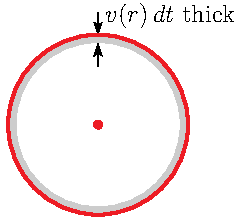
\includegraphics{waterField2.pdf}
\end{center}
\end{efig}}
During a very short time interval $dt$ seconds, $4\pi m\,dt$ litres
of water is created at the origin (which is the red dot). As the water 
is incompressible, $4\pi m\,dt$ litres of water must exit through 
the sphere during the same time interval to make room for the newly 
created water. 

But, at the surface of the sphere the water is flowing radially outward 
with speed $v(r)$. So during the time interval in question the water near the surface of
the sphere moves outward a distance $v(r)\,dt$, and in particular the water 
that was in the thin spherical shell 
$\ \ r-v(r)\,dt \le \sqrt{x^2+y^2+z^2} \le r\ \ $ at the beginning of 
the time interval exits through the sphere $\sqrt{x^2+y^2+z^2} = r$ 
during the time interval. The shell is sketched in gray in the figure 
above. The volume of water in the gray shell is essentially the surface 
area of the shell, which is $4\pi r^2$, times the thickness of the 
shell, which is $v(r)\,dt$. So, equating the volume of water created inside 
the sphere with the volume of water that exited the sphere,
\begin{equation*}
4\pi m\,dt =  (4\pi r^2) \big(v(r)\,dt\big)
\implies v(r) = \frac{4\pi m}{4\pi r^2} =\frac{m}{r^2}
\end{equation*}
Thus our vector field is
\begin{equation*}
\vv(x,y,z) = \frac{m}{r(x,y,z)^2}\,\hat\vr(x,y,z)
\end{equation*}
If the world were two, rather than three dimensional\footnote{You might want to think about what happens in $d$ dimensions for general $d$.}, and the source
created $2\pi m$ litres per second, the same argument leads to
\begin{equation*}
2\pi m\,dt =  (2\pi r) \big(v(r)\,dt\big)
\implies v(r) = \frac{2\pi m}{2\pi r} =\frac{m}{r}
\end{equation*}
and to the vector field
\begin{equation*}
\vv(x,y) = \frac{m}{r(x,y)}\,\hat\vr(x,y)\qquad
r(x,y) = \sqrt{x^2+y^2}\qquad
\hat\vr(x,y) = \frac{x\hi + y\hj}{\sqrt{x^2+y^2}}
\end{equation*}
To get a mental image of what this field looks like, imagine
sketching, for each point $(x,y)$, the vector  
$\frac{m}{r(x,y)}\,\hat\vr(x,y)$ with its tail at
$(x,y)$. Note that the vector  $\frac{m}{r(x,y)}\,\hat\vr(x,y)$ 
\begin{itemize}\itemsep1pt \parskip0pt \parsep0pt %\itemindent-15pt
\item[$\circ$]
points radially outward and
\item[$\circ$]
has length $\frac{m}{r(x,y)}$ which
\begin{itemize}\itemsep1pt \parskip0pt \parsep0pt %\itemindent-15pt
\item[$\circ$]
depends only on $r=|(x,y)|$ and
\item[$\circ$]
is very long when $(x,y)$ is near the origin and
\item[$\circ$]
decreases in length like $\frac{1}{r}$ as $r=|(x,y)|$ increases.
\end{itemize}
\end{itemize}
Here is a sketch of a bunch of such vectors.
\begin{fig}\label{fig:sourceField}
\begin{center}
    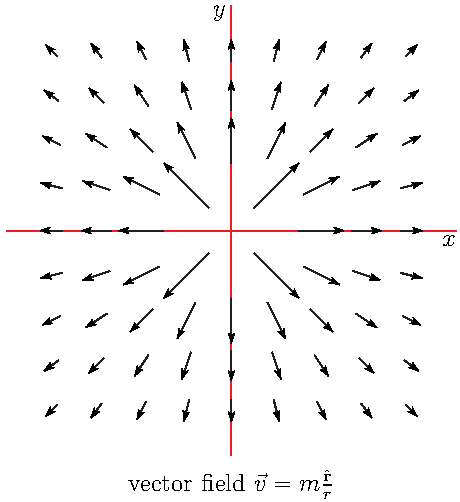
\includegraphics{waterField.pdf}
\end{center}
\end{fig}
\noindent
Note that as $|(x,y)|\rightarrow 0$, the magnitude of the velocity 
$|\vv(x,y)|\rightarrow\infty$. This is a consequence of our idealized
assumption that we are producing water at a single point (the origin).
\end{eg}


\begin{eg}[The Vortex]\label{eg:Vortex}
In this example, we sketch the vector field
\begin{equation*}
\vv(x,y) = \Om\big(-y\hi +x\hj\big)
\end{equation*}
where $\Om$ is just a strictly positive constant.
We give an efficient procedure for getting a rough sketch, which still
provides a pretty realistic picture of the vector field, and which also
generalises to other vector fields.
First concentrate
on the horizontal component $\hi\cdot\vv(x,y)$ of the vector field and 
determine in which part of the $xy$-plane it is zero, in which part 
it is positive and in which part it is negative.
\begin{equation*}
\hi\cdot\vv(x,y)
=-\Om y\ \ 
\begin{cases}
   =0 &\text{if $y=0$}\\
   <0 &\text{if $y>0$}\\
   >0 &\text{if $y<0$}
\end{cases}
\end{equation*}
Next repeat with the vertical component.
\begin{equation*}
\hj\cdot\vv(x,y)
= \Om x\ \ 
\begin{cases}
   =0 &\text{if $x=0$}\\
   <0 &\text{if $x<0$}\\
   >0 &\text{if $x>0$}
\end{cases}
\end{equation*}
This naturally divides the $xy$-plane into nine parts according to whether
each of the components is positive, $0$ or negative --- 
\begin{itemize}\itemsep1pt \parskip0pt \parsep0pt %\itemindent-15pt
\item[$\circ$]
$\hi\cdot\vv>0$ and $\hj\cdot\vv>0$
in $\big\{\ (x,y)\in\bbbr^2\ \big|\  y<0,\ x>0\ \big\}$ 
\item[$\circ$]
$\hi\cdot\vv>0$ and $\hj\cdot\vv=0$
in $\big\{\ (x,y)\in\bbbr^2\ \big|\  y<0,\ x=0\ \big\}$ 
\item[$\circ$]
$\hi\cdot\vv>0$ and $\hj\cdot\vv<0$
in $\big\{\ (x,y)\in\bbbr^2\ \big|\  y<0,\ x<0\ \big\}$ 
\item[$\circ$]
$\hi\cdot\vv=0$ and $\hj\cdot\vv>0$
in $\big\{\ (x,y)\in\bbbr^2\ \big|\  y=0,\ x>0\ \big\}$ 
%\item[$\circ$]
%$\hi\cdot\vv=0$ and $\hj\cdot\vv=0$
%in $\big\{\ (x,y)\in\bbbr^2\ \big|\  y=0,\ x=0\ \big\}$ 
%\item[$\circ$]
%$\hi\cdot\vv=0$ and $\hj\cdot\vv<0$
%in $\big\{\ (x,y)\in\bbbr^2\ \big|\  y=0,\ x<0\ \big\}$ 
%\item[$\circ$]
%$\hi\cdot\vv<0$ and $\hj\cdot\vv>0$
%in $\big\{\ (x,y)\in\bbbr^2\ \big|\  y>0,\ x>0\ \big\}$ 
%\item[$\circ$]
%$\hi\cdot\vv<0$ and $\hj\cdot\vv=0$
%in $\big\{\ (x,y)\in\bbbr^2\ \big|\  y>0,\ x=0\ \big\}$ 
%\item[$\circ$]
%$\hi\cdot\vv<0$ and $\hj\cdot\vv<0$
%in $\big\{\ (x,y)\in\bbbr^2\ \big|\  y>0,\ x<0\ \big\}$ 
\item[$\circ$] 
and so on
\end{itemize}
Now think of $\vv(x,y)$ as being the velocity at $(x,y)$ of a flowing fluid.
\begin{itemize}%\itemsep1pt \parskip0pt \parsep0pt %\itemindent-15pt
\item[$\circ$]
Look at the first bullet point above. It says that in the first of the nine 
parts, namely $\big\{\ (x,y)\in\bbbr^2\ \big|\  y<0,\ x>0\ \big\}$,
which is the fourth quadrant, 
the horizontal component  $\hi\cdot\vv>0$ signifying that the fluid is flowing
rightwards. Indicate this in the sketch by drawing a rightward pointing 
horizontal arrow at some generic point in the middle of the fourth quadrant. 
(It's the blue arrow in the figure below.)
The vertical component  $\hj\cdot\vv>0$ signifying that the fluid is 
also moving upwards. Indicate this in the sketch by drawing an upward 
pointing vertical arrow at the same generic point in the fourth quadrant.
(It's the red arrow in the figure below.)
\begin{efig}
\begin{center}
    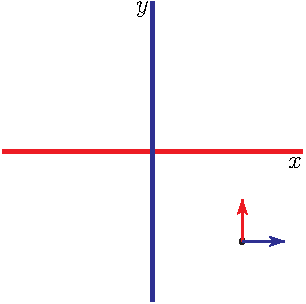
\includegraphics{phaseVortex4.pdf}
\end{center}
\end{efig}


\item[$\circ$]
Next, look at the second bullet point above. It says that on the second of the nine parts, namely $\big\{\ (x,y)\in\bbbr^2\ \big|\  y<0,\ x=0\ \big\}$,
which is the bottom half of the $y$-axis, 
the horizontal component  $\hi\cdot\vv>0$, signifying that the fluid is moving
rightwards. Indicate this in the sketch by drawing a rightward pointing 
horizontal arrow at some generic point in the middle of the bottom half 
of the $y$-axis. (It's the second blue arrow in the figure below.) 
The vertical component  $\hj\cdot\vv=0$ signifying that the fluid has
no vertical motion at all. Indicate this in the sketch by not drawing any 
vertical arrow on the bottom half of the $y$-axis.
\begin{efig}
\begin{center}
    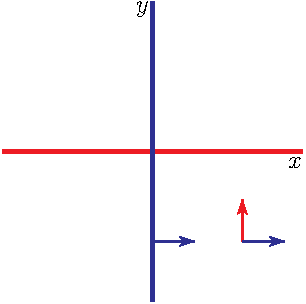
\includegraphics{phaseVortex5.pdf}
\end{center}
\end{efig}


\item[$\circ$]
and so on

\end{itemize}
By the time we have looked at all nine regions we will have built up the
following sketch.
\begin{fig}\label{fig:vortexCrude}
\begin{center}
    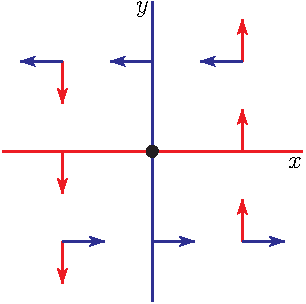
\includegraphics{phaseVortex1.pdf}
\end{center}
\end{fig}
\noindent
From this sketch we see that, for example, in the first quadrant, 
the fluid is moving upwards and to the left. We also see that there is one 
point, namely $(0,0)$, where the vector field is exactly zero. It's the
black dot in the centre of the figure above.
Putting all of this 
accumulated wisdom together, and also noticing that $\vv(x,y)$ is smaller 
when $(x,y)$ is closer to the origin and $\vv(x,y)$ is larger when 
$(x,y)$ is farther from the origin, we come up with this better 
sketch of the vector field.
\begin{fig}\label{fig:vortexField}
\begin{center}
    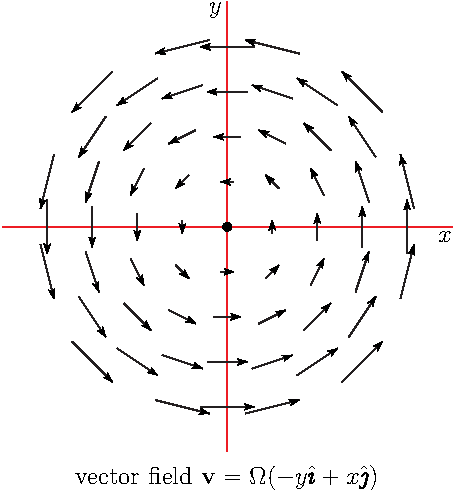
\includegraphics{vortexField.pdf}
\end{center}
\end{fig}
\noindent
This shows the field swirling around the origin in a counterclockwise direction.
Hence the name ``vortex''.
\end{eg}



\begin{eg}[The Undamped Nonlinear Pendulum]\label{eg:Pendulum}
In this example, we illustrate another way in which  vector fields
arise. Model a pendulum by a mass $m$ that is connected to a hinge by 
an idealized rod that is massless\footnote{While we are idealizing, let's put
everything in a vacuum.} and of fixed length $\ell$. Denote 
by $\theta$ the angle
\vadjust{
\begin{efig}
\begin{center}
    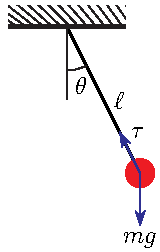
\includegraphics{pendulum3.pdf}
\end{center}
\end{efig}
}
between the rod and vertical. The forces acting on the mass are
\begin{itemize}\itemsep1pt \parskip0pt \parsep0pt %\itemindent-15pt
\item[$\circ$]
gravity and
\item[$\circ$]
the tension in the rod, whose magnitude, $\tau$, automatically adjusts 
itself so that the distance between the mass and the hinge is 
fixed at $\ell$. 
\end{itemize}
In the optional\footnote{In the optional Section \ref{sec:Pendulum} we also
include frictional forces. In this example, we do not, so set the $\beta$
of Section \ref{sec:Pendulum} to zero here.} Section \ref{sec:Pendulum}, 
we show that the angle $\theta(t)$ obeys the second order 
nonlinear\footnote{It is common, when considering only small amplitude 
oscillations, to approximate $\sin\theta$ by $\theta$. This converts our
nonlinear differential equation into a linear differential equation.} 
differential equation
\begin{equation*}
\difftwo{\theta}{t} +\frac{g}{\ell}\sin\theta=0
\end{equation*}
It is often much more convenient to deal with first order, rather than
second order, differential equations.
The second order pendulum equation above may be 
reformulated\footnote{This ``hack'' generalizes easily and is 
commonly used when generating, by computer, approximate solutions to higher order ordinary differential equations.} 
as a system of first order ordinary differential equations, by the 
simple expedient of defining
\begin{equation*}
x(t)=\theta(t)\qquad y(t)=\theta'(t)
\end{equation*}
So $x(t)$ is the angle at time $t$ and $y(t)$ is the angular velocity at time $t$. Then, 
\begin{alignat*}{3}
x'(t)&=&\theta'(t)&=y(t)\cr
y'(t)&=&\ \theta''(t)&=-\frac{g}{\ell}\sin x(t)
\end{alignat*}
Usually, one does not write in the $(t)$ dependence explicitly.
\begin{align*}
x'&=y\cr
y'&=-\frac{g}{\ell}\sin x
\end{align*}
The right hand sides form the vector field
\begin{equation*}
\vv\big((x,y)\big)=\Big(y\,,\,-\frac{g}{\ell}\sin x\Big)
\end{equation*}
We can sketch this vector field, just as we sketched the vector field 
of Example \ref{eg:Vortex}. Noting that the horizontal component
\begin{equation*}
\hi\cdot\vv(x,y)
= y\ \ 
\begin{cases}
   =0 &\text{if $y=0$}\\
   >0 &\text{if $y>0$}\\
   <0 &\text{if $y<0$}
\end{cases}
\end{equation*}
and the vertical component.
\begin{equation*}
\hj\cdot\vv(x,y)
= -\frac{g}{\ell}\sin x\ \ 
\begin{cases}
   =0 &\text{if $x=0,\ \pm\pi, \pm2\pi, \cdots$}\\
   >0 &\text{if $-\pi<x<0$,\ \  $\pi<x<2\pi$, etc.}\\
   <0 &\text{if $0<x<\pi$, \ \ $2\pi<x<3\pi$, etc.}
\end{cases}
\end{equation*}
we have
\begin{itemize}\itemsep1pt \parskip0pt \parsep0pt %\itemindent-15pt
\item[$\circ$]
rightward motion\footnote{Note that this is rightward motion of the point $(x,y)$, not of the pendulum itself.} when $y>0$
\item[$\circ$]
leftward motion when $y<0$
\item[$\circ$]
downward motion when $0<x<\pi$,\ \  $2\pi<x<3\pi$, $\cdots$ and 
\item[$\circ$]
upward motion when $-\pi<x<0$,\ \  $\pi<x<2\pi$, $\cdots$. 
\end{itemize}
This gives us the collection of arrows in the figure
\begin{wfig}
\begin{center}
    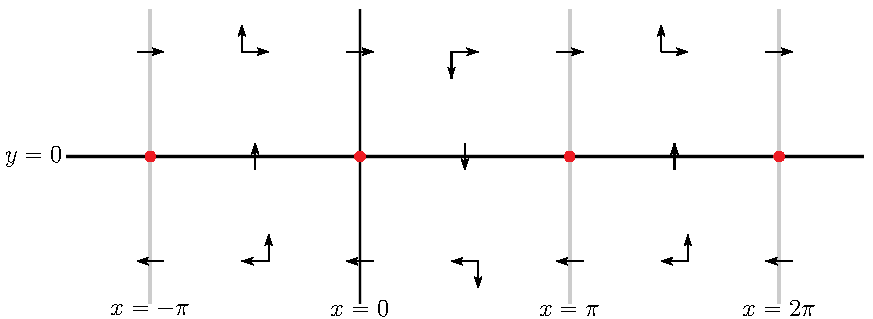
\includegraphics{phasePendulum1.pdf}
\end{center}
\end{wfig}
Our full sketch will be less cluttered if we make all arrows the
same length. This gives
\begin{wfig}
\begin{center}
    \null\hskip0.3in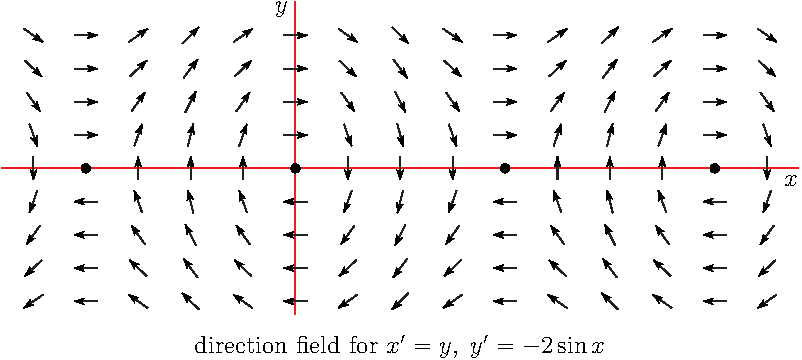
\includegraphics{pendulumField2.pdf}
\end{center}
\end{wfig}
which is a sketch of what is called the direction field of our vector field
(see below). 

In the next section, we'll learn how to use vector field sketches to sketch solution trajectories.
\end{eg}

\begin{defn}\label{def:VFdirnFld}
The direction field of a vector field $\vv(x,y,z)$ is the vector field
\begin{equation*}
\vV(x,y,z) =\begin{cases}
   \frac{\vv(x,y,z)}{|\vv(x,y,z)|} &\text{if $\vv(x,y,z)\ne\vZero$} \\[0.1in]
     \vZero & \text{if $\vv(x,y,z) = \vZero$}
\end{cases}
\end{equation*}
\end{defn}

\section{Optional --- Field Lines}\label{sec:fieldLines}
%\section{Field Lines}\label{sec:fieldLines}

Suppose that we drop a tiny stick into a river\footnote{Think Poohsticks.
%chip logs
} with the velocity
field of the flowing water being $\vv(x,y)$. We are assuming, for 
simplicity, that the velocity field does not depend\footnote{This is not such an unreasonable assumption. The flow often changes on a larger time scale.} 
on time $t$. The stick will move along with the 
water\footnote{This is also not an unreasonable approximation.}. When the stick 
is at $\vr$, its velocity will be the same as the velocity of the 
water at $\vr$, which is $\vv(\vr)$. Thus if the stick is at 
$\vr(t)$ at time $t$, we will have
\begin{equation*}
\diff{\vr}{t} = \vv\big(\vr(t)\big)
\end{equation*}
The stick will trace out a path, parametrized by $\vr(t)$. 

\begin{defn}\label{def:fieldLine} 
A path that is parametrized by a function $\vr(t)$ that obeys
\begin{equation*}
\diff{\vr}{t} = \vv\big(\vr(t)\big)
\end{equation*}
is called a
\begin{itemize}\itemsep1pt \parskip0pt \parsep0pt %\itemindent-15pt
\item[$\circ$] field line or integral curve (for general vector fields) or a
\item[$\circ$] stream line or flow line (when the vector field $\vv$ is
                  being thought of as a velocity field) or a
\item[$\circ$] line of force (when the vector field $\vv$ is
                  being thought of as a force field)
\end{itemize}
of the vector field $\vv$.
\end{defn}

\begin{eg}[Flow Line Sketch for the Vortex of Example \ref{eg:Vortex}]
\label{eg:flowSketchVortex}
Consider the vortex vector field, $\vv(x,y) = \Om\big(-y\hi +x\hj\big)$ 
of Example \ref{eg:Vortex}. Once we sketched the vector field, as in
Figure \ref{fig:vortexField}, or even made the ``skeleton sketch'' of
Figure \ref{fig:vortexCrude}, we can get rough idea of what the stream lines 
look like just by following the arrows. For example, suppose that
we start a stream line (i.e. drop the stick into the stream) on the positive
$x$-axis. Looking at Figure \ref{fig:vortexCrude}, which is repeated
here,

\begin{efig}
\begin{center}
    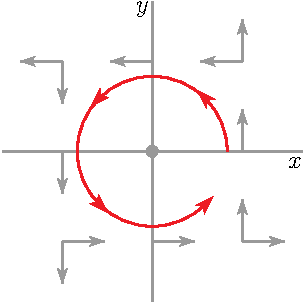
\includegraphics{phaseVortex2.pdf}
\end{center}
\end{efig}

\noindent the stick 
\begin{itemize}\itemsep1pt \parskip0pt \parsep0pt %\itemindent-15pt
\item[$\circ$]
starts by moving in the $+y$ direction, i.e. straight upward.
\item[$\circ$]
As it moves farther into the first quadrant it develops
a larger and larger negative $x$-component of velocity.
So it also moves leftwards toward the $y$-axis.  
\item[$\circ$]
Eventually it crosses the positive $y$-axis moving in the $-x$ direction,
i.e. to the left.
\item[$\circ$]
As it moves farther into the second quadrant it develops
a larger and larger negative $y$-component of velocity.
So it also moves downwards toward the $x$-axis.
\item[$\circ$]
Eventually it crosses the negative $x$-axis moving in the $-y$ direction, 
i.e. straight downward.
\item[$\circ$]
As it moves farther into the third quadrant it develops
a larger and larger positive $x$-component of velocity.
So it also moves rightward towards the $y$-axis.
\item[$\circ$]
Eventually it crosses the negative $y$-axis moving in the $+x$ direction,
i.e. to the right.
\item[$\circ$]
As it moves farther into the fourth quadrant it develops
a larger and larger positive $y$-component of velocity.
So it also moves upwards toward the $x$-axis.
\end{itemize}
With this type of analysis we cannot tell if the streamline, which is the red 
line in the figure above, will return to the $x$-axis 
\begin{itemize}\itemsep1pt \parskip0pt \parsep0pt %\itemindent-15pt
\item[$\circ$]
exactly at its starting point, forming a closed curve, or
\item[$\circ$]
inside its starting point, spiralling inwards, or
\item[$\circ$]
outside its starting point, spiralling outwards.
\end{itemize}
\end{eg}

While the above procedure is a good way to get a qualitative feel 
for trajectories,
we can develop more precise, detailed descriptions of field lines by
working analytically. As we saw above, thinking of $\vr(t)$ as the position
at time $t$ of a stick dropped into water whose velocity at $(x,y)$ is $\vv(x,y)$, the velocity of the stick at time $t$ will be the same 
as the velocity of the  water at $\vr(t)$, which is $\vv\big(\vr(t)\big)$. 
Thus $\vr(t)$ will obey the system of first order differential equations
\begin{impeqn}\label{eq:VFstreamLineA}
\begin{equation*}
\diff{\vr}{t}(t) = \vv\big(\vr(t)\big) 
\end{equation*}
\end{impeqn}

Notice that if we reparametrize $\vr(t)$, say to $\vR(u) = \vr\big(t(u)\big)$,
then $\vR'(u) =   \vr'\big(t(u)\big)\ t'(u)$ is parallel to
(though not necessarily equal to) $\vr'\big(t(u)\big)= \vv\big(\vr\big((t(u)\big)\big)
                         =\vv\big(\vR(u)\big)$. 
So if we only care about the curve traced out by the stick, and not about 
\emph{when} the stick is at each point of the path, then it suffices to
impose the weaker condition\footnote{We'll have a more careful discussion of 
this in the optional \S\ref{sec:fieldLinePara}.} that, when the stick 
is at $\vr(t)$, its velocity $\vr'(t)$ is parallel to (though not necessarily equal to) 
$\vv\big(\vr(t)\big)$. In three dimensions, $\vr'(t)$ is parallel to 
$\vv\big(\vr(t)\big)$ when the cross product is zero:
\begin{impeqn}\label{eq:VFstreamLineBB}
\begin{equation*}
\vr'(t)\times\vv\big(\vr(t)\big)=\vZero
\end{equation*}
\end{impeqn}
\noindent
In two dimensions we can still use the cross product by the simple
expedient of thinking of $\vr'(t)$ and $\vv\big(\vr(t)\big)$ as three component
vectors whose third components are zero. 


A more convenient way to implement the weaker ``just parallel'' 
condition, involves reparametrizing our streamline. 
Suppose that we are in two dimensions 
with $\vr'(t)=\big(\diff{x}{t}(t)\,,\,\diff{y}{t}(t)\big)$ and
$\vv(\vr)=\big(v_1(\vr)\,,\,v_2(\vr)\big)$  and fix some $t_0$. If $\diff{x}{t}(t_0)$ is 
nonzero\footnote{If $\diff{x}{t}(t_0)=0$,
but $\diff{y}{t}(t_0)\ne 0$, we should use $y$ rather than $x$ as the 
parameter. If $\diff{x}{t}(t_0)=\diff{y}{t}(t_0)=0$, then $\vr(t)=\vr(t_0)$
for all $t$ and the streamline doesn't move. It is just a single point.}, 
we can reparametrize the curve (at least near $\vr(t_0)$) so as to use $x$, rather than $t$ as the parameter. To do so, we
\begin{itemize}\itemsep1pt \parskip0pt \parsep0pt %\itemindent-15pt
\item[$\circ$] solve $x=x(t)$ for $t$ as a function of $x$. Call 
the solution $T(x)$. Then
\item[$\circ$] the point on the curve which has $x$-coordinate $x$ is 
$\vR(x)=\big(X(x)\,,\,Y(x)\big)$ with $X(x)=x$ and $Y(x) = y\big(T(x)\big)$. 
\end{itemize}
Then the condition that $\vR'(x)=\big(1,Y'(x)\big)$ is parallel to $\vv\big(\vR(x)\big)$ says that $\vR'(x)$ is a scalar multiple of
$\vv\big(\vR(x)\big)$ so that 
there is a nonzero number $c(x)$ so that $\vR'(x)=c(x) \vv\big(\vR(x)\big)$. That is
\begin{equation*}
\big(1,Y'(x)\big) 
   =\big( c(x)v_1\big(x,Y(x)\big)\,,\, c(x)v_2\big(x,Y(x)\big)  \big)
\end{equation*}
or equivalently
\begin{equation*}
Y'(x)=\frac{Y'(x)}{1}
=\frac{c(x)\,v_2\big(x,Y(x)\big)}{c(x)\,v_1\big(x,Y(x)\big)\big)}
=\frac{v_2\big(x,Y(x)\big)}{v_1\big(x,Y(x)\big)}
\end{equation*}
This is exactly the statement that $y=Y(x)$ is a solution of the differential equation
\begin{equation*}
\diff{y}{x}(x) = \frac{v_2\big(x,y\big)}{v_1\big(x,y\big)}
\end{equation*}
It is conventional to pretend\footnote{Of course $\diff{y}{x}$ is not the ratio of $\dee{y}$ and $\dee{x}$. However pretending that it is provides a simple
way to remember the technique that is used to solve the equation. You have used this mnemonic device before when you learned how to solve separable differential equations.} 
that $\diff{y}{x}$ is the ratio of $\dee{y}$ and $\dee{x}$ and rewrite the differential equation\footnote{Here is another nonrigorous, but intuitive way
to come up with this equation. Suppose that our stick is at $(x,y)$ 
and has velocity $\big(\diff{x}{t}(t)\,,\,\diff{y}{t}(t)\big)$. 
In a tiny time interval $\dee{t}$ the stick moves by $\big(\diff{x}{t}(t)\,,\,\diff{y}{t}(t)\big)\dee{t}
=(\dee{x},\dee{y})$, which is parallel to  $\big(v_1(x,y)\,,\,v_2(x,y)\big)$
if $\frac{\dee{x}}{v_1(x,y)}=\frac{\dee{y}}{v_2(x,y)}$.} as
\begin{equation*}
\frac{\dee{x}}{v_1(x,y)}=\frac{\dee{y}}{v_2(x,y)}
\end{equation*}

Here is a summary of the discussion we have just completed. It extends to three dimensions in an obvious way.
\begin{impeqn}\label{eq:VFstreamLineB}
Use the symbol $\parallel$ to stand for ``is parallel to''.

\noindent
In two dimensions
\begin{align*}
&\Big(\diff{x}{t}(t)\,,\,\diff{y}{t}(t)\Big) \parallel
\big(v_1(\vr(t))\,,\,v_2(\vr(t)\big) \\
&\hskip0.5in\iff  
\Big(\diff{x}{t}(t)\,,\,\diff{y}{t}(t)\,,\,0\Big)\times
\big(v_1(\vr(t))\,,\,v_2(\vr(t))\,,\,0\big) = \vZero \\
&\hskip0.5in\iff \frac{dx}{v_1(x,y)}=\frac{dy}{v_2(x,y)}
\end{align*}
and in three dimensions 
\begin{align*}
&\Big(\diff{x}{t}(t)\,,\,\diff{y}{t}(t)\,,\,\diff{z}{t}(t)\Big) \parallel
\big(v_1(\vr(t))\,,\,v_2(\vr(t))\,,\,v_3(\vr(t))\big) \\
&\hskip0.5in\iff  
\Big(\diff{x}{t}(t)\,,\,\diff{y}{t}(t)\,,\,\diff{z}{t}(t)\Big)\times
\big(v_1(\vr(t))\,,\,v_2(\vr(t))\,,\,v_3(\vr(t))\big) = \vZero \\
&\hskip0.5in\iff \frac{dx}{v_1(x,y,z)}=\frac{dy}{v_2(x,y,z)}=\frac{dz}{v_3(x,y,z)}
\end{align*}
\end{impeqn}
Let us apply this to two examples, in which the stream lines of the vortex field 
of Example \ref{eg:Vortex} are found by two different methods.

\begin{eg}[Stream lines for the vortex field using 
                             $\vr'(t)\parallel\vv(\vr(t))$]
             \label{eg:vortexStreamParallel}
 In this example we will find the stream lines for the vortex field, 
$\vv(x,y) = \Om\big(-y\hi +x\hj\big)$ of Example \ref{eg:Vortex},
by using the requirement that, on a stream line, the velocity vector
$\vr'(t)$ must be parallel to $\vv\big(\vr(t)\big)$. 
By \eqref{eq:VFstreamLineB} one way to express this requirement mathematically is
\begin{align*}
\frac{dx}{-\Om y} = \frac{dy}{\Om x}
\end{align*}
This is a simple separable differential equation. We can solve it 
by cross multiplying and integrating both sides. (Recall that $\Om$ is a 
constant.)
\begin{align*}
\Om x\,\dee{x} = -\Om y\,\dee{y}
&\iff \Om \int x\,\dee{x} = -\Om \int y\,\dee{y} \\
&\iff \half \Om x^2 =-\half \Om y^2 +C' \\
&\iff x^2+y^2 = C
\end{align*}
where $C'$ and $C=\frac{2}{\Om}C'$ are just arbitrary constants. So the stream lines of the vortex field are exactly circles centred on the origin.
\begin{efig}
\begin{center}
    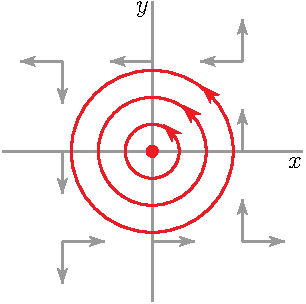
\includegraphics{phaseVortex3.pdf}
\end{center}
\end{efig}


We can come to exactly the same conclusion by using the cross product 
formulation of \eqref{eq:VFstreamLineBB}.
\begin{align*}
&\Big(\diff{x}{t}(t)\,,\,\diff{y}{t}(t)\,,\,0\Big)\times
\big(v_1(\vr(t))\,,\,v_2(\vr(t))\,,\,0\big) = \vZero \\
&\hskip0.5in\iff \Big(\diff{x}{t}(t)\,\hi+\diff{y}{t}(t)\,\hj\Big)\times
\big(-\Om y(t)\,\hi+\Om x(t)\,\hj\big) = \vZero \\
&\hskip0.5in\iff \Big(\Om x(t)\diff{x}{t}(t) 
               +\Om y(t)\diff{y}{t}(t)\Big)\hk=\vZero \\
&\hskip0.5in\iff \Om x(t)\diff{x}{t}(t) 
               +\Om y(t)\diff{y}{t}(t)=0 \\
&\hskip0.5in\iff \diff{\ }{t}\Big(\half \Om x(t)^2+\half\Om y(t)^2\Big)=0 
\qquad\text{(Go ahead and evaluate the derivative.)}\\
&\hskip0.5in\iff \half\Om\big(x(t)^2+y(t)^2\big) = C' \\
&\hskip0.5in\iff x(t)^2+y(t)^2=C
\end{align*}
\end{eg}

\begin{eg}[Stream lines for the vortex field
using $\vr'(t)=\vv(\vr(t))$]\label{eg:vortexStreamEqual}
This time we will find the stream lines for the vortex field, 
$\vv(x,y) = \Om\big(-y\hi +x\hj\big)$ of Example \ref{eg:Vortex},
by using \eqref{eq:VFstreamLineA}, which is
\begin{align*}
\diff{x}{t} &= -\Om y \\
\diff{y}{t} &= \Om x 
\end{align*}
We can convert this system of first
order linear ordinary differential equations
into a single second order linear constant coefficient
differential equation\footnote{In Example \ref{eg:Pendulum} we converted a second order ordinary differential equation into a system of first
order ordinary differential equations. We are now just reversing
the procedure we used there.}, by differentiating 
the first equation, to get $\difftwo{x}{t} = -\Om\diff{y}{t}$,
and then substituting in the second equation to get
\begin{equation*}
\difftwo{x}{t} + \Om^2 x = 0
\end{equation*}
This equation is a special case of the ordinary differential equation
treated in Example \ref{eg:RLC} of the Appendix \ref{ap:ODE}, entitled
``Review of Linear Ordinary Differential Equations''.  In fact it is
exactly (\ref{eqn:ODERy}$_{\rm h}$) with $R=0$, $L=C=\frac{1}{\Om}$. So
the general solution is \eqref{eqn:RLCampPhase} with 
$\rho=0$ and $\nu=\Om$, which is
\begin{equation*}
x(t) = A\cos(\Om t-\theta)
\end{equation*} 
with $A$ and $\theta$ being arbitrary constants\footnote{Even if you
don't know how $x(t) = A\cos(\Om t-\theta)$ was arrived at, you should
be able to easily verify that it really does obey $x''+\Om^2 x=0$.}. Then
\begin{equation*}
y(t) = -\frac{1}{\Om}\diff{x}{t} =A\sin(\Om t-\theta)
\end{equation*}
giving us the familiar circular stream lines.
\end{eg}

\subsection{More about $\vr'(t)\times\vv\big(\vr(t)\big)=\vZero$}
            \label{sec:fieldLinePara}
Here is a lemma that gives a more precise version of
``if we only care about the curve traced out by the stick, and not about 
when the stick is at each point of the path, then it suffices to
impose the weaker condition 
$\vr'(t)\times\vv\big(\vr(t)\big)=\vZero$''.
\begin{lemma}\label{lem:fieldLinePara}
Lat $a<b$ and let $\vv(\vr)$ be a vector field. Assume that,
for all $a<u<b$,  $\vR(u)$ is defined, both $\vR'(u)$ and 
$\vv\big(\vR(u)\big)$ are continuous and  nonzero and
\begin{equation*}
\vR'(u)\times\vv\big(\vR(u)\big)=\vZero
\end{equation*}
Then $\Set{\vR(u)}{a<u<b}$ is contained in a field line.
\end{lemma}
\begin{proof}
As $\vR'(u)\times\vv\big(\vR(u)\big)=\vZero$ and  both 
$\vR'(u)$ and $\vv\big(\vR(u)\big)$ are nonzero,  there is 
an $a(u)$ such that
\begin{equation*}
\vR'(u) = a(u)\,\vv\big(\vR(u)\big)
\end{equation*} 
This $a(u)=\frac{\vR'(u)\cdot\vv(\vR(u))}{\vv(\vR(u))\cdot\vv(\vR(u))}$ 
is necessarily nonzero and continuous. Since $a(u)$ is nonzero and continuous,
it never changes sign. That is, either $a(u)>0$ for all  $u$,
or $a(u)<0$ for all $u$. Let $T(u)$ be an antiderivative of $a(u)$. Then $T(u)$
is strictly monotone (and continuous) and hence invertible. That is, there 
is a continuous function $U(t)$ that obeys $U\big(T(u)\big)=u$ for all 
$a<u<b$ and $T\big(U(t)\big)=t$ for all $t$ in the range of $U$. Set 
$\vr(t) = \vR\big(U(t)\big)$.
Then
\begin{align*}
\vr'(t) &= \vR'\big(U(t)\big) U'(t)
        = a\big(U(t)\big)\,\vv\big(\vR\big(U(t)\big)\big)
                                    \frac{1}{T'\big(U(t)\big)}
        = a\big(U(t)\big)\,\vv\big(\vr(t)\big)
                                    \frac{1}{a\big(U(t)\big)} \\
        &=\vv\big(\vr(t)\big)
\end{align*}
So $\vr(t)$ is a field line and $\vR(u) = \vr(T(u))$ 
is a reparametrization of $\vr(t)$.
\end{proof}

Here are a couple of examples that show that bad things can happen
if we drop the requirement that $\vv(\vR(u))$ is nonzero.

\begin{eg}\label{ex:badStreamA}
Let the vector field $\vv(x,y)$ be identically zero. Then any field line
$\big(x(t)\,,\,y(t)\big)$ must obey
\begin{align*}
x'(t)=0\qquad y'(t)=0
\end{align*}
which forces both $x(t)$ and $y(t)$ to be constants. So each field line is
just a single point. On the other hand every nonconstant
$\vR(u)$ obeys $\vR'(u)\times\vv\big(\vR(u)\big)=\vZero$ but is not 
contained in a field line.
\end{eg}

Now here is a more interesting example.

\begin{eg}\label{ex:badStreamB}
Consider the vector field $\vv(x,y)=x\,\hi$. This vector field takes the value $\vZero$ at each point on the $y$-axis, is a positive multiple of $\hi$
at every point of the right half-plane and is a negative multiple of 
$\hi$ at every point of the left half-plane. Let's find the field lines.
Any field line must obey
\begin{align*}
\diff{x}{t}(t)=x(t)\qquad \diff{y}{t}(t)=0
\end{align*}
So $y(t)$ must be a constant. We can solve the linear ordinary
differential equation $\diff{x}{t}(t)=x(t)$ by moving
the $x(t)$ to the left hand side, and multiplying by the (integrating factor)
$e^{-t}$. This gives
\begin{equation*}
e^{-t}\diff{x}{t}(t)-e^{-t} x(t)=0
\end{equation*}
By the product rule, this is the same as
\begin{equation*}
\diff{\hfill}{t}\big(e^{-t}x(t)\big)=0
\end{equation*}
which forces $e^{-t}x(t)$ to be a constant. So our field lines are
$\big(Ce^t\,,\,D\big)$, with $C$ and $D$ being arbitrary constants.
Note that
\begin{itemize}
\item
if $C=0$, the field line is just the single point $(0,D)$ on the $y$-axis.
It is illustrated by the black dot in the figure below.

\item
If $C>0$, then as $t$ runs from $-\infty$ to $+\infty$, the field line
covers the horizontal half-line
\begin{equation*}
\Set{(x,D)}{x>0}
\end{equation*}
in the right half-plane.
It is illustrated by the red line in the figure below.


\item
If $C<0$, then as $t$ runs from $-\infty$ to $+\infty$, the field line
covers the horizontal half-line
\begin{equation*}
\Set{(x,D)}{x<0}
\end{equation*}
in the left half-plane.
It is illustrated by the blue line in the figure below.


\end{itemize}

\begin{nfig}
\begin{center}
   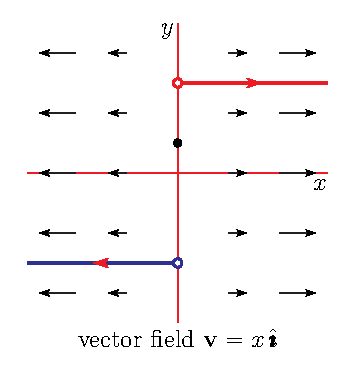
\includegraphics{horizontalField}
\end{center}
\end{nfig}
On the other hand, fix any constant $D$ and set $\vR(u) = u\hi +D\hj$.
Then
\begin{equation*}
\vR'(u)\times\vv\big(\vR(u)\big)
=\hi\times\big(u\hi)
=\vZero
\end{equation*}
But as $u$ runs from $-\infty$ to $+\infty$, $\vR(u)$ runs over the 
full line $\Set{(x,D)}{-\infty<x<\infty}$. It is not contained in any
single field line and, in fact, completely covers three
different field lines. 


\end{eg}

\section{Conservative Vector Fields}\label{sec:conservativeFields}

Not all vector fields are created equal. In particular, some vector
fields are easier to work with than others. One important class 
of vector fields that are relatively easy to work with, at least sometimes, 
but that still arise in many applications are ``conservative vector fields''. 

\begin{defn}\label{def:conservative}

\begin{enumerate}[(a)]
\item
The vector field $\vF$ is said to be \emph{conservative} if there
exists a function $\varphi$ such that $\vF = \vnabla\varphi$. Then
$\varphi$ is called a \emph{potential} for $\vF$. Note that if $\varphi$ 
is a potential for $\vF$ and if $C$ is a constant, then $\varphi+C$
is also a potential for $\vF$.

\item If $\vF=\vnabla\varphi$ is a conservative field with potential 
$\varphi$ and if $C$ is a constant, then the set of points that
obey $\varphi(x,y,z)=C$ is called an equipotential surface.
Similarly, in two dimensions, the set of points that
obey $\varphi(x,y)=C$ is called an equipotential curve.
\end{enumerate}
\end{defn}

\begin{warning}\label{warn:potential}
In physics,  when a vector field is of the form $\vF=-\vnabla\varphi$,
then $\varphi$ is called a potential for $\vF$.
\emph{Note} the minus\footnote{Physicists introduce this minus sign in order to eliminate the minus sign in the next footnote.} sign in 
%  $\vF=\textcolor{blue}{\mathbf{-}}\vnabla\varphi$. 
  $\vF=\underset{\uparrow}{-}\vnabla\varphi$. 
\end{warning}

\begin{eg}[Potential energy]\label{eg:potentialEnergy}
The ``conservative'' in ``conservative vector field'' has nothing
to do with politics. It comes from ``conservation of energy''.
Here is how. Suppose that you have a particle of mass $m$ moving in
a force field $\vF$ that happens to be of the form $\vF=\vnabla\varphi$
for some function $\varphi$. 
If the position of the particle a time $t$ is $\big(x(t),y(t),z(t)\big)$,
then, by Newton's law of motion,
\begin{alignat*}{3}
 m\va = \vF \qquad
&\implies & m\diff{\vv}{t}(t) &= \vF\big(x(t),y(t),z(t)\big) \\
&\implies & m\diff{\vv}{t}(t) &= \vnabla\varphi\big(x(t),y(t),z(t)\big)\\
\intertext{Now dot both sides with $\vv(t)$.} 
&\implies & m\,\vv(t)\cdot\diff{\vv}{t}(t) &= \vv(t)\cdot\vnabla\varphi\big(x(t),y(t),z(t)\big)  \\
& & &=x'(t)\frac{\partial\varphi}{\partial x}\big(x(t),y(t),z(t)\big)
+y'(t)\frac{\partial\varphi}{\partial y}\big(x(t),y(t),z(t)\big) \\
& & & \hskip1in
+z'(t)\frac{\partial\varphi}{\partial z}\big(x(t),y(t),z(t)\big)\\
\intertext{Next use $\diff{\ }{t}\vv\cdot\vv=2\vv\cdot\diff{\vv}{t}$
on the left hand side and the chain rule on the right hand side.}
&\implies &\ \ \diff{\ }{t}\Big(\frac{1}{2} m \vv(t)\cdot\vv(t)\Big) 
    &= \diff{\ }{t}\Big(\varphi\big(x(t),y(t),z(t)\big)\Big) \\
&\implies &  &\hskip-1.3in\diff{\ }{t}\Big(\frac{1}{2} m \vv(t)\cdot\vv(t) 
    -\varphi\big(x(t),y(t),z(t)\big)\Big) =0 \\[0.1in]
&\implies &  &\hskip-1.0in\frac{1}{2} m |\vv(t)|^2
    -\varphi\big(x(t),y(t),z(t)\big) = \text{const}
\end{alignat*}
So $\frac{1}{2} m |\vv(t)|^2
    -\varphi\big(x(t),y(t),z(t)\big)$, which is called the 
energy\footnote{$\frac{1}{2} m |\vv(t)|^2$ is the kinetic energy and
$-\varphi$ is the potential energy. See Warning \ref{warn:potential}.}  of the 
particle at time $t$, does not actually depend on time --- it is conserved.
Let's call the initial energy $E$. That is,
$E=\frac{1}{2} m |\vv(0)|^2 -\varphi\big(x(0),y(0),z(0)\big)$.
Then $\frac{1}{2} m |\vv(t)|^2 -\varphi\big(x(t),y(t),z(t)\big)=E$
for all $t$ and, in particular
\begin{equation*}
\varphi\big(x(t),y(t),z(t)\big) = \frac{1}{2} m |\vv(t)|^2 -E
             \ge -E
\end{equation*}
So even without having to find $\big(x(t)\,,\,y(t)\,,\,z(t)\big)$,
we know that our particle can never escape the region 
$\Set{(x,y,z)}{\varphi(x,y,z)\ge -E}$.
\end{eg}


\begin{eg}[Gravity]\label{eg:gravity}
The gravitational force that a body of mass $M$ at the origin
exerts on a body of mass $m$ at $\vr=(x,y,z)$ is
\begin{equation*}
\vF(\vr) = -\frac{GMm}{r^3}\vr
\end{equation*}
where $r=|\vr|=\sqrt{x^2+y^2+z^2}$ and $G$ is the gravitational constant.
This force is conservative, with potential $\varphi(\vr) = \frac{GMm}{r}$. 
To verify that this is correct, observe that
\begin{alignat*}{3}
\frac{\partial\ }{\partial x}\varphi(\vr)
   &=\frac{\partial\ }{\partial x}\frac{GMm}{\sqrt{x^2+y^2+z^2}}
   &=-\frac{1}{2}\frac{GMm(2x)}{[x^2+y^2+z^2]^{3/2}} 
   &=-\frac{GMm}{r^3}x \\ 
\frac{\partial\ }{\partial y}\varphi(\vr)
   &=\frac{\partial\ }{\partial y}\frac{GMm}{\sqrt{x^2+y^2+z^2}}
   &=-\frac{1}{2}\frac{GMm(2y)}{[x^2+y^2+z^2]^{3/2}} 
   &=-\frac{GMm}{r^3}y \\ 
\frac{\partial\ }{\partial z}\varphi(\vr)
   &=\frac{\partial\ }{\partial z}\frac{GMm}{\sqrt{x^2+y^2+z^2}}
   &=-\frac{1}{2}\frac{GMm(2z)}{[x^2+y^2+z^2]^{3/2}} 
   &=-\frac{GMm}{r^3}z  
\end{alignat*}
\end{eg}

We have already found conservation of energy very helpful 
a couple of times in Section \ref{sec:Sliding} (Sliding on a Curve).
So, at this point, there are probably several questions gnawing away at you.
\begin{itemize}
\item
Is every vector field conservative?

\item
If not, is there an easy way to tell whether or not a vector field 
is conservative?

\item
If we know that a given vector field is conservative, how do find a potential
for it?

\end{itemize}
Have no fear. We will consider those questions in some detail shortly.
But first, a couple of more examples. 



\begin{eg}\label{eg:fieldlinesPotential}
In this example we will show that the vector field $\vF(x,y) = x\,\hi-y\,\hj$
is conservative and find both its potential and its field lines.
\begin{enumerate}[(a)]
\item \emph{The potential:}\ \ \ Our vector field $\vF(x,y) = x\,\hi-y\,\hj$
is conservative if we can find a $\varphi$ obeying
\begin{align*}
\frac{\partial \varphi}{\partial x}(x,y) &= x \\
\frac{\partial \varphi}{\partial y}(x,y) &= -y 
\end{align*}
Recall that, when taking the partial derivative $\frac{\partial\ }{\partial x}$
the coordinate $y$ is viewed as a constant. So the first of these equations
is satisfied if and only if there is a $\psi(y)$, which does not depend on $x$,
so that 
\begin{equation*}
\varphi(x,y) = \frac{x^2}{2} +\psi(y)
\end{equation*}
For this to also satisfy the second equation, we need
\begin{align*}
-y=\frac{\partial \varphi}{\partial y}(x,y)
=\frac{\partial\ }{\partial y}\Big(\frac{x^2}{2} +\psi(y)\Big)
=\psi'(y)
\end{align*}
which is the case if and only if there is a constant $C$ with
\begin{equation*}
\psi(y) =-\frac{y^2}{2} +C
\end{equation*}
So, for any choice of the constant $C$,
\begin{equation*}
\frac{x^2}{2} - \frac{y^2}{2} +C
\end{equation*}
is a potential. In particular, taking $C=0$, one possible potential is 
\begin{equation*}
\varphi(x,y) = \frac{x^2}{2} - \frac{y^2}{2}
\end{equation*}
Some equipotential curves for this potential are sketched in (c) below. 
They are the blue curves.

\item
\emph{The field lines (Optional):}\ \ \
Recalling \eqref{eq:VFstreamLineB},
the field lines of the vector field $\vF(x,y) = x\,\hi-y\,\hj$
are determined by
\begin{align*}
\frac{\dee{x}}{x} = \frac{\dee y}{-y}
&\iff -y\dee x = x\dee{y} \\
&\iff x\dee{y} + y\dee x = 0 \\
&\iff \dee{(xy)} = 0 \qquad\text{by the product rule} \\
&\iff xy = C
\end{align*}
for some constant $C$. If you are not comfortable with the use
of the product rule above, here is another way to write the
same computation.
\begin{align*}
\diff{y}{x}=-\frac{y}{x}
&\iff  x\diff{y}{x} = -y \\
&\iff x\diff{y}{x} +y = 0 \\
&\iff \diff{\hfill}{x}(xy) = 0 \qquad\text{by the product rule} \\
&\iff xy = C
\end{align*}
Some field lines are sketched in (c) below.
They are the red curves. Note that they appear to cross the equipotential 
curves, the blue curves, at right angles. We shall see in 
Lemma \ref{lem:equipotential}, below, that this is not a coincidence.
Also note that, while the above computation tells what the field lines
are, it does not give us the direction of motion along the field lines.
We determine the direction of motion next. 

\item 
\emph{Direction of motion (Optional):}\ \ \ 
The sign data
\begin{align*}
\hi\cdot\vF(x,y) = x
    \left.\begin{cases}
             >0 &\text{if $x>0$} \\
             =0 &\text{if $x=0$} \\
             <0 &\text{if $x<0$} 
       \end{cases}\right\}\qquad
\hj\cdot\vF(x,y) = -y
    \left.\begin{cases}
             >0 &\text{if $y<0$} \\
             =0 &\text{if $y=0$} \\
             <0 &\text{if $y>0$} 
       \end{cases}\right\}\qquad
\end{align*}
is visually displayed in the figure on the left below. The arrows in the
figure on the left gives us the direction of motion along 
the field lines (in red) in the figure on the right below.
Some equipotential curves are also sketched (in blue) in the figure 
on the right below.

\begin{efig}
\begin{center}
    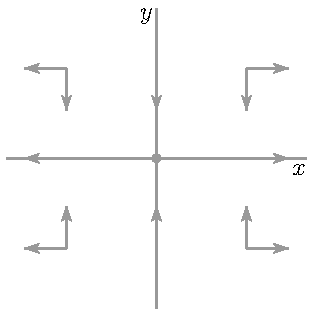
\includegraphics{phaseHyperbola.pdf}\qquad
    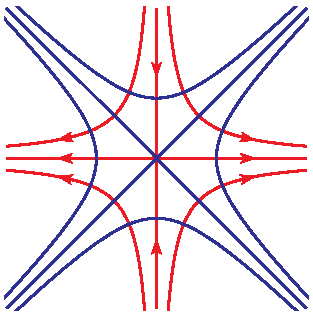
\includegraphics{phaseHyperbola3.pdf}
\end{center}
\end{efig}

\end{enumerate}
\end{eg}


We have just seen one example of a conservative vector field for which the
field lines appear to cross the equipotential curves at right angles.
Here is a result which says that that was no accident. The field lines of
conservative fields always cross the equipotential surfaces 
at right angles. 

\begin{lemma}[Optional]\label{lem:equipotential}
If $\vF$ is a conservative vector field, then the field lines of $\vF$
are perpendicular to the equipotential surfaces of $\vF$.
\end{lemma}
\begin{proof}
Let $\vF=\vnabla\varphi$. 
Pick any point $\vr_0$ and any nonzero vector $\vT$ 
that is tangent to the equipotential surface at $\vr_0$. That
equipotential surface is  $\varphi\big(x,y,z\big)=\varphi(\vr_0)$.
Consider any curve $\vr(t)=\big(x(t),y(t),z(t)\big)$ that 
\begin{itemize}\itemsep1pt \parskip0pt \parsep0pt %\itemindent-15pt
\item[$\circ$]
lies in the equipotential surface of $\vF$ through $\vr_0$,
so that $\varphi\big(\vr(t)\big)=\varphi(\vr_0)$ for all $t$, 
and also obeys
\item[$\circ$]
$\vr(0)=\vr_0$ and
\item[$\circ$]
$\diff{\vr}{t}(0) = \vT$.
\end{itemize}
Differentiating $\varphi\big(\vr(t)\big)=\varphi(\vr_0)$
with respect to $t$ and applying the chain rule gives
\begin{align*}
\diff{\ }{t}\big[\varphi\big(x(t),y(t),z(t)\big)\big] &=0 \\
\frac{\partial\varphi}{\partial x}\big(x(t),y(t),z(t)\big)\diff{x}{t}(t)
+\frac{\partial\varphi}{\partial y}\big(x(t),y(t),z(t)\big)\diff{y}{t}(t)
+\frac{\partial\varphi}{\partial z}\big(x(t),y(t),z(t)\big)\diff{z}{t}(t)
&=0 
\end{align*}
Notice that the left hand side is exactly the dot product
of $\big(\frac{\partial\varphi}{\partial x}
\,,\,\frac{\partial\varphi}{\partial y}
\,,\,\frac{\partial\varphi}{\partial z}\big)=\vnabla\varphi$ 
with
$\big(\diff{x}{t}
\,,\,\diff{y}{t}
\,,\,\diff{z}{t}\big)
=\diff{\vr}{t}$.
So
\begin{align*}
\vnabla\varphi\big(\vr(t)\big)\cdot\diff{\vr}{t}(t) &= 0 \\
 \vF\big(\vr(t)\big)\cdot\diff{\vr}{t}(t) &= 0
\end{align*}
Then set $t=0$ to get
\begin{equation*}
 \vF\big(\vr_0\big)\cdot\vT = 0
\end{equation*}
This says that the vector $\vT$ (which is tangent to the equipotential 
surface at $\vr_0$) is perpendicular 
to the vector field at $\vr_0$ (which is a tangent vector to the 
field line of $\vF$ through $\vr_0$).
\end{proof}

Here is another example in which we try to find a potential for a vector field.

\begin{eg}\label{eg:potentialB}
Let's try to find a potential for the vortex vector field
$\vv(x,y) = \Om\big(-y\hi +x\hj\big)$ of Example \ref{eg:Vortex}.
The potential would have to obey
\begin{align*}
\frac{\partial \varphi}{\partial x}(x,y) &= -\Om y \\
\frac{\partial \varphi}{\partial y}(x,y) &= \Om x 
\end{align*}
We proceed just as we did in Example \ref{eg:fieldlinesPotential}.
The first of these equations is satisfied if and only if there is a 
$\psi(y)$, which does not depend on $x$, so that 
\begin{equation*}
\varphi(x,y) = -\Om xy +\psi(y)
\end{equation*}
For this to also satisfy the second equation, we need
\begin{align*}
\Om x=\frac{\partial \varphi}{\partial y}(x,y)
=\frac{\partial\ }{\partial y}\Big(-\Om xy +\psi(y)\Big)
=-\Om x +\psi'(y)
\iff \psi'(y) = 2\Om x
\end{align*}
If $\Om\ne 0$, the right hand side of this equation depends on $x$
while the left hand side in independent of $x$, no matter what $\psi$ is.
So no $\psi$ can work, and $\vv(x,y) = \Om\big(-y\hi +x\hj\big)$ is not 
conservative. 
\end{eg}

The previous example shows that not all vector fields are conservative.
That answers the first of the questions that we posed just before Example
\ref{eg:fieldlinesPotential}.
The next theorem provides a simple screening test for conservativeness,
which partially answers the second question. The easy way to remember the
screening test uses the curl, which we now define.

\begin{defn}\label{def:curl}
The curl of a vector field $\vF(x,y,z)$ is denoted by $\vnabla\times\vF(x,y,z)$
and is defined by
\begin{align*}
\vnabla\times\vF
&=\Big(\frac{\partial F_3}{\partial y} -\frac{\partial F_2}{\partial z} \Big)\hi
+\Big(\frac{\partial F_1}{\partial z} -\frac{\partial F_3}{\partial x} \Big)\hj
+\Big(\frac{\partial F_2}{\partial x} -\frac{\partial F_1}{\partial y} \Big)\hk
\\
&=\det\left[\begin{matrix}
                \hi &\hj & \hk \\
                \frac{\partial\ }{\partial x} & \frac{\partial\ }{\partial y}
                      & \frac{\partial\ }{\partial z} \\
                F_1(x,y,z) & F_2(x,y,z) & F_3(x,y,z)
            \end{matrix}\right]
\end{align*}
The determinant in the second row is really just a mnemonic device
used to make it easy to remember the expression after the equals sign 
in the first row. One must be careful about the signs in this definition ---
the determinant helps with that.

\end{defn}




\begin{theorem}[Screening test for conservative vector fields.]
   \label{thm:screen}
\begin{enumerate}[(a)]
\item
Assume that $F_1(x,y)$ and $F_2(x,y)$ are continuously differentiable.
If the vector field $F_1(x,y)\hi + F_2(x,y)\hj$ is conservative, then
we must have
\begin{equation*}
\frac{\partial F_1}{\partial y} =  \frac{\partial F_2}{\partial x}
\end{equation*}

\item
Assume that $F_1(x,y,z)$, $F_2(x,y,z)$ and $F_3(x,y,z)$ are continuously differentiable.
If the vector field $F_1(x,y,z)\hi + F_2(x,y,z)\hj + F_3(x,y,z)\hk$ is conservative, then
\begin{equation*}
\frac{\partial F_1}{\partial y} =  \frac{\partial F_2}{\partial x}\qquad
\frac{\partial F_1}{\partial z} =  \frac{\partial F_3}{\partial x}\qquad
\frac{\partial F_2}{\partial z} =  \frac{\partial F_3}{\partial y}
\end{equation*}
Equivalently,
\begin{equation*}
\vnabla\times\vF 
=\Big(\frac{\partial F_3}{\partial y} -\frac{\partial F_2}{\partial z} \Big)\hi
+\Big(\frac{\partial F_1}{\partial z} -\frac{\partial F_3}{\partial x} \Big)\hj
+\Big(\frac{\partial F_2}{\partial x} -\frac{\partial F_1}{\partial y} \Big)\hk
  =\vZero
\end{equation*}
That is, $\vF$ is curl free.

\end{enumerate}
\end{theorem}

\begin{proof}
(a) 
If the vector field $F_1(x,y)\hi + F_2(x,y)\hj$ is conservative,
then there is a potential $\varphi(x,y)$ such that
\begin{align*}
\frac{\partial \varphi}{\partial x}(x,y) &= F_1(x,y) \\
\frac{\partial \varphi}{\partial y}(x,y) &= F_2(x,y) 
\end{align*}
Applying $\frac{\partial\ }{\partial y}$ to the first equation and 
$\frac{\partial\ }{\partial x}$ to the second equation gives
\begin{align*}
\frac{\partial^2 \varphi}{\partial y\partial x}
       &= \frac{\partial F_1}{\partial y} \\
\frac{\partial^2 \varphi}{\partial x\partial y}
       &= \frac{\partial F_2}{\partial x} 
\end{align*}
Recall that, for any twice continuously differentiable function,
$\frac{\partial^2 \varphi}{\partial y\partial x} =
\frac{\partial^2 \varphi}{\partial x\partial y}$.
So the two left hand sides are equal, 
and the two right hand sides must also be equal.

\noindent (b) 
If the vector field $F_1(x,y,z)\hi + F_2(x,y,z)\hj + F_3(x,y,z)\hk$ 
is conservative, then there is a potential $\varphi(x,y,z)$ such that
\begin{align*}
\frac{\partial \varphi}{\partial x}(x,y,z) &= F_1(x,y,z) \\
\frac{\partial \varphi}{\partial y}(x,y,z) &= F_2(x,y,z) \\
\frac{\partial \varphi}{\partial z}(x,y,z) &= F_3(x,y,z) 
\end{align*}
We proceed just as in (a).
\begin{itemize}\itemsep1pt \parskip0pt \parsep0pt %\itemindent-15pt 
\item Applying
$\frac{\partial\ }{\partial y}$ to the first equation and 
$\frac{\partial\ }{\partial x}$ to the second equation gives
\begin{align*}
\left\{\atp{  \frac{\partial^2 \varphi}{\partial y\partial x}
                    = \frac{\partial F_1}{\partial y}  }
             {  \frac{\partial^2 \varphi}{\partial x\partial y}
                  = \frac{\partial F_2}{\partial x} }\right\}
\implies \frac{\partial F_1}{\partial y} = \frac{\partial F_2}{\partial x} 
\end{align*}
\item Applying
$\frac{\partial\ }{\partial z}$ to the first equation and 
$\frac{\partial\ }{\partial x}$ to the third equation gives
\begin{align*}
\left\{\atp{  \frac{\partial^2 \varphi}{\partial z\partial x}
                    = \frac{\partial F_1}{\partial z}  }
             {  \frac{\partial^2 \varphi}{\partial x\partial z}
                  = \frac{\partial F_3}{\partial x} }\right\}
\implies \frac{\partial F_1}{\partial z} = \frac{\partial F_3}{\partial x} 
\end{align*}
\item Applying
$\frac{\partial\ }{\partial z}$ to the second equation and 
$\frac{\partial\ }{\partial y}$ to the third equation gives
\begin{align*}
\left\{\atp{  \frac{\partial^2 \varphi}{\partial z\partial y}
                    = \frac{\partial F_2}{\partial z}  }
             {  \frac{\partial^2 \varphi}{\partial y\partial z}
                  = \frac{\partial F_3}{\partial y} }\right\}
\implies \frac{\partial F_2}{\partial z} = \frac{\partial F_3}{\partial y} 
\end{align*}

\end{itemize}
Combining the three bullet points gives $\vnabla\times\vF=\vZero$.
\end{proof}

\begin{warning}\label{warn:screening}
As always, we have to be careful with the flow of logic\footnote{
Use your favourite search engine to look up a list of common logical
errors. One is ``affirming the consequent''. An example would be concluding 
that because Shakespeare is dead, Elvis, who is also dead, 
must also be Shakespeare.}.
The screening test in Theorem \ref{thm:screen} is a one-way test.
If, for example, 
$\frac{\partial F_1}{\partial y}~\ne~\frac{\partial F_2}{\partial x}$
then the vector field $\vF$ cannot be conservative. But if
$\frac{\partial F_1}{\partial y} =  \frac{\partial F_2}{\partial x}$
Theorem \ref{thm:screen} does \emph{not} guarantee that
$\vF$ is conservative. In fact there are fields that are not conservative
but do obey $\frac{\partial F_1}{\partial y}=\frac{\partial F_2}{\partial x}$.
We'll see one in Example \ref{eg:screeningCounterexample}, below.  
We shall later find some additional regularity conditions which, when 
combined with $\frac{\partial F_1}{\partial y}=\frac{\partial F_2}{\partial x}$,
do imply conservativeness. See Theorem \ref{thm:screenConserv}, below.
\end{warning}


\begin{eg}[Example \ref{eg:potentialB} revisited]\label{eg:potentialBB}
In Example \ref{eg:potentialB}, we attempted to find a potential 
for the vector field 
\begin{equation*}
\vv(x,y) = \Om\big(-y\hi +x\hj\big)
\end{equation*}
In the end we showed that, if $\Om\ne 0$, no potential could exist, i.e. 
$\vv(x,y)$ is not conservative. Had we known
the screening test of Theorem \ref{thm:screen}.a, we could have
concluded that $\vv(x,y)$ is not conservative by simply observing that
\begin{alignat*}{3}
\frac{\partial \vv_1}{\partial y}&= \frac{\partial \ }{\partial y}\big(-\Om y) &= -\Om \\
\frac{\partial \vv_2}{\partial x}&= \ \ \frac{\partial \ }{\partial x}\big(\Om x) &= +\Om
\end{alignat*}
are not equal, unless $\Om=0$. But $\Om=0$ makes a rather boring vector 
field.
\end{eg}


\begin{eg}\label{eg:potentialC}
Determine whether or not the vector field
\begin{equation*}
\vF(x,y,z) = y\hi -z\hj +x\hk
\end{equation*}
is conservative. If it is conservative, find a potential.

\soln
Let's start by applying the screening test Theorem \ref{thm:screen}.b.
Since
\begin{align*}
\vnabla\times\vF
&=\det\left[\begin{matrix}
                \hi &\hj & \hk \\
                \frac{\partial\ }{\partial x} & \frac{\partial\ }{\partial y}
                      & \frac{\partial\ }{\partial z} \\
                y & -z & x
            \end{matrix}\right]
=\hi-\hj-\hk
\end{align*}
is not $\vZero$, the vector field $\vF$ cannot be conservative.
\end{eg}


\begin{eg}\label{eg:potentialD}
Determine whether or not the vector field
\begin{equation*}
\vF(x,y,z) = (y^2+2xz^2-1)\hi +(2x+1)y\,\hj +(2x^2z+z^3)\hk
\end{equation*}
is conservative. If it is conservative, find a potential.

\soln
Again start by applying the screening test Theorem \ref{thm:screen}.b.
This time
\begin{align*}
\vnabla\times\vF
&=\det\left[\begin{matrix}
                \hi &\hj & \hk \\
                \frac{\partial\ }{\partial x} & \frac{\partial\ }{\partial y}
                      & \frac{\partial\ }{\partial z} \\
                y^2+2xz^2-1 & (2x+1)y & 2x^2z+z^3
            \end{matrix}\right]
=0\hi-(4xz-4xz)\hj+(2y-2y)\hk \\
=\vZero
\end{align*}
So $\vF$ passes the screening test. Let's look for a function 
$\varphi(x,y,z)$ obeying
\begin{align}
\frac{\partial \varphi}{\partial x}(x,y,z) &= y^2+2xz^2-1 \notag\\
\frac{\partial \varphi}{\partial y}(x,y,z) &= (2x+1)y \tag{$*$}\\
\frac{\partial \varphi}{\partial z}(x,y,z) &= 2x^2z+z^3 \notag
\end{align}
The partial derivative $\frac{\partial \ }{\partial x}$ treats $y$
and $z$ as constants. So $\varphi(x,y,z)$ obeys the first equation
if and only if there is a function $\psi(y,z)$ with
\begin{equation*}
\varphi(x,y,z)
=xy^2+x^2z^2-x
+\psi(y,z)
\end{equation*}
This $\varphi(x,y,z)$ will also obey the second equation if and only if 
\begin{align*}
\frac{\partial \ }{\partial y}\big(xy^2+x^2z^2-x+\psi(y,z)\big) = (2x+1)y
&\iff 2xy +\frac{\partial\psi}{\partial y}(y,z) = (2x+1)y \\
&\iff \frac{\partial\psi}{\partial y}(y,z) = y \\
&\iff \psi(y,z) = \frac{y^2}{2} +\zeta(z)
\end{align*}
for some function $\zeta(z)$ which depends only on $z$. At this stage
we know that 
\begin{equation*}
\varphi(x,y,z)
=xy^2+x^2z^2-x+\psi(y,z)
=xy^2+x^2z^2-x+\frac{y^2}{2}+\zeta(z)
\end{equation*}
obeys the first two equations of ($*$),
for any function $\zeta(z)$. Finally to have the third equation of 
($*$) also satisfied, we also need to chose $\zeta(z)$
to obey
\begin{align*}
\frac{\partial \ }{\partial z}\big(xy^2+x^2z^2-x+\frac{y^2}{2}+\zeta(z)\big) 
 = 2x^2z+z^3 
&\iff 2x^2z +\zeta'(z) = 2x^2z + z^3 \\
&\iff \zeta'(z) = z^3\\
&\iff \zeta(z) = \frac{z^4}{4} + C
\end{align*}
for any constant $C$. So one possible potential, namely that with $C=0$ is
\begin{equation*}
\varphi(x,y,z)
=xy^2+x^2z^2-x+\frac{y^2}{2}+\frac{z^4}{4}
\end{equation*}
Note, as a check\footnote{It is always worth doing this check.}, that
\begin{equation*}
\vnabla \varphi(x,y,z)
=\big(y^2+2xz^2-1\big)\hi+\big(2xy+y)\hj+\big(2x^2z+z^3\big)\hk
\end{equation*}
as desired.
\end{eg}

\begin{eg}[Optional: First look at $-\frac{y}{x^2+y^2}\hi + \frac{x}{x^2+y^2}\hj$]\label{eg:screeningCounterexample}
Now is a good time to reread the Warning \ref{warn:screening}.
In this example we will show that the vector field
\begin{equation*}
\vF(x,y) = -\frac{y}{x^2+y^2}\hi + \frac{x}{x^2+y^2}\hj
\qquad \text{defined for all $(x,y)$ in $\bbbr^2$ except $(x,y)=(0,0)$}
\end{equation*}
passes the screening test of Theorem \ref{thm:screen}.a. We will also
begin to see why it is \emph{not} conservative on the domain
$\bbbr^2\setminus\{(0,0)\}$. To verify the screening test, we compute
\begin{alignat*}{3}
\frac{\partial\ }{\partial y}\Big(-\frac{y}{x^2+y^2}\Big)
  &= -\frac{(x^2+y^2) - y(2y)}{{(x^2+y^2)}^2} 
  &&= \frac{y^2-x^2}{{(x^2+y^2)}^2} \\
\frac{\partial\ }{\partial x}\Big(\frac{x}{x^2+y^2}\Big)
  &=\phantom{-} \frac{(x^2+y^2) - x(2x)}{{(x^2+y^2)}^2} 
  &&= \frac{y^2-x^2}{{(x^2+y^2)}^2}
\end{alignat*}
and observe that the two right hand sides are identical. So the
screening test is passed.

In order for $\vF$ to be conservative on the domain
$\bbbr^2\setminus\{(0,0\}$, there must exist a function
$\varphi(x,y)$, that, together with both partial derivatives 
$\frac{\partial \varphi}{\partial x}(x,y)$ and 
$\frac{\partial \varphi}{\partial y}(x,y)$, is defined for all $(x,y)$ 
in $\bbbr^2$ except $(x,y)=(0,0)$, and obeys
\begin{alignat*}{3}
\frac{\partial \varphi}{\partial x}(x,y) &= -\frac{y}{x^2+y^2}
&&= \frac{-\frac{y}{x^2}}{1+\big(\frac{y}{x}\big)^2}
&&=\frac{\partial\ }{\partial x}\Big(\arctan\frac{y}{x}\Big) \\
\frac{\partial \varphi}{\partial y}(x,y) &= \phantom{-} \frac{x}{x^2+y^2} 
&&= \frac{\frac{1}{x}}{1+\big(\frac{y}{x}\big)^2}
&&=\frac{\partial\ }{\partial y}\Big(\arctan\frac{y}{x}\Big)
\end{alignat*}
by the chain rule, because
\begin{equation*}
\frac{\partial\ }{\partial x}\Big(\frac{y}{x}\Big) =-\frac{y}{x^2}
\qquad
\frac{\partial\ }{\partial y}\Big(\frac{y}{x}\Big)=\frac{1}{x}
\end{equation*}
It looks like we have found a potential, namely $\arctan\frac{y}{x}$.
But there is a problem. Recall that, by definition, $\arctan\frac{y}{x}$ is 
an angle $\theta(x,y)$ that obeys
$\tan\theta(x,y)= \arctan\frac{y}{x}$; but for any 
$(x,y)\in\bbbr^2\setminus\{(0,0\}$ there are infinitely many angles 
having the tangent $\frac{y}{x}$. To define $\varphi(x,y)$ we have to 
select exactly one such angle. It is impossible to do so in such a way 
that $\varphi(x,y)$ is continuous on all of $\bbbr^2\setminus\{(0,0\}$.

To see why, fix any $r>0$, and imagine that you are walking on the circle
$x^2+y^2=r^2$ in the $xy$-plane. At time $\theta$, you are at $x=r\cos\theta$,
$y=r\sin\theta$ and then $\frac{y}{x} = \tan\theta$ and you are allowed to 
define $\varphi(x,y)=\theta+k\pi$, for any integer $k$.

 Suppose that at time $\theta=0$ you choose $k=0$. That is, you choose $\varphi(r,0)=0$.
Now start walking, choosing an allowed $\varphi(x,y)$, i.e. choosing a $k$, 
for each point $(x,y)$ that you cross.
Because $\varphi(x,y)$ has to vary continuously\footnote{If $\varphi(x,y)$
is not continuous, its gradient does not exist, and $\varphi$ cannot be 
a potential.} with $(x,y)$, you 
have to continue choosing $k=0$. But you run off a cliff as $\theta$ 
approaches $2\pi$, because then
\begin{itemize}
\item[$\circ$] 
you are approaching $(r,0)$ from below, as in the figure below, and
\item[$\circ$]
because you are choosing $k=0$, $\varphi(x,y)$ is just a little less than 
$2\pi$, but
\item[$\circ$]
you have already chosen $\varphi(r,0)=0$, not $2\pi$.
So $\varphi(x,y)$ has a jump discontinuity\footnote{Those who have taken
some complex analysis may recognize this as the branch cut in $\ln z$.} 
along the positive $x$-axis.
\end{itemize}
\begin{efig}
\begin{center}
    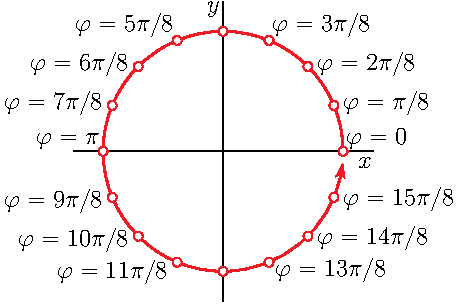
\includegraphics{notConservative.pdf}
\end{center}
\end{efig}
If you are having trouble following this argument, don't worry about it.
We will return with a less hand-wavy argument later.
\end{eg}


\section{Line Integrals}\label{sec:workIntegrals}
We have already seen, in \S\ref{sec:lineIntegral}, one type of integral along
curves. We are now going to see a second, that turns out to have significant
connections to conservative vector fields. It arose from the concept of 
``work'' in classical mechanics. 

Suppose that we wish to find the work done
%, from time $t_0$ to time $t_1$, 
by a force $\vF(\vr)$ moving a particle 
along a path $\vr(t)$. During the ``infinitesimal time interval\footnote{Yes, yes. We should first consider short time intervals $\De t>0$ and then take the limit 
$\De t\rightarrow 0$ at the end. But you have undoubtedly used this 
type of argument so many times before that you would be thoroughly 
bored by it.}'' 
from $t$ to $t+\dee{t}$  the particle moves from $\vr(t)$ to $\vr(t)+\dee{\vr}$ with $\dee{\vr}=\diff{\vr}{t}(t)\,\dee{t}$. By definition, the work done 
during that infinitesimal time interval is 
\begin{equation*}
\vF\big(\vr(t)\big)\cdot\dee{\vr} = \vF\big(\vr(t)\big)\cdot
\diff{\vr}{t}(t)\,\dee{t}
\end{equation*}
The total work done during the time interval from $t_0$ to $t_1$ is then
\begin{equation*}
\text{Work} = \int_{t_0}^{t_1}\vF\big(\vr(t)\big)\cdot\diff{\vr}{t}(t)\,\dee{t}
\end{equation*}
There are some useful shorthand notations for this work.

\begin{notn}\label{not:workIntegral}
Denote by $\cC$ the parametrized path $\vr(t)$ with $t_0\le t\le t_1$. 
Then
\begin{equation*}
\int_\cC\vF\cdot\dee{\vr}
=\int_\cC\big(\vF_1\dee{x}+\vF_2\dee{y}+\vF_3\dee{z}\big)
=\int_{t_0}^{t_1}\vF\big(\vr(t)\big)\cdot\diff{\vr}{t}(t)\,\dee{t}
\end{equation*}
If $\cC$ is a closed path, the notation $\oint_\cC\vF\cdot\dee{\vr}$
is also used.
\end{notn}

In the event that $\vF$ is conservative, and we know the potential $\varphi$,
the following theorem provides a really easy way to compute
``work integrals''. The theorem is a generalization of the fundamental theorem 
of calculus, and indeed some people call it the fundamental theorem of line integrals.
\begin{theorem}\label{thm:workIntegral}
Let $\vF=\nabla\varphi$ be a conservative vector field. Then if $\cC$ is
any curve that starts at $P_0$ and ends at $P_1$, we have\footnote{So $\varphi$
acts a bit like the antiderivative of first year calculus.}
\begin{equation*}
\int_\cC\vF\cdot\dee{\vr} =\varphi(P_1)-\varphi(P_0)
\end{equation*}
\end{theorem}
\begin{proof}
Let $\vr(t)=\big(x(t),y(t),z(t)\big)$, $t_0\le t\le t_1$, 
be any parametrization of $\cC$ with $\vr(t_0)=P_0$ and $\vr(t_1)=P_1$. 
Then, by definition,
\begin{align*}
\int_\cC\vF\cdot\dee{\vr}
&=\int_{t_0}^{t_1}\vF\big(\vr(t)\big)\cdot\diff{\vr}{t}(t)\,\dee{t}
=\int_{t_0}^{t_1}\vnabla\varphi\big(\vr(t)\big)\cdot\diff{\vr}{t}(t)\,\dee{t}
\\
&=\int_{t_0}^{t_1}\Big[
\frac{\partial\varphi}{\partial x}\big(x(t),y(t),z(t)\big)
                        \diff{x}{t}(t)
+\frac{\partial\varphi}{\partial y}\big(x(t),y(t),z(t)\big)
                        \diff{y}{t}(t) \\&\hskip3in
+\frac{\partial\varphi}{\partial z}\big(x(t),y(t),z(t)\big)
                        \diff{z}{t}(t) 
\Big]\dee{t} \\
&=\int_{t_0}^{t_1}\diff{\ }{t}\Big[\varphi\big(x(t),y(t),z(t)\big)
\Big]\dee{t} 
\qquad\text{by the chain rule in reverse}\\
&=\varphi\big(\vr(t_1)\big) - \varphi\big(\vr(t_0)\big)
=\varphi(P_1) - \varphi(P_0)
\end{align*}
by the fundamental theorem of calculus.
\end{proof}
Observe that, in Theorem \ref{thm:workIntegral}, the value,
$\varphi(P_1)-\varphi(P_0)$, of the integral $\int_\cC\vF\cdot\dee{\vr}$
depended only on the endpoints $P_0$ and $P_1$ of the curve, not on the path 
that the curve followed to get to $P_0$ from $P_1$. We shall see, in Theorem
\ref{thm:pathIndepConserv}, below, that this happens only for 
conservative vector fields.
Here are several examples of line integrals of vector fields that are not
conservative.


\begin{eg}\label{eg:workIntegalA}
Set $P_0=(0,0)$, $P_1=(1,1)$ and\footnote{The reader should check that this
vector field is not conservative.}
\begin{equation*}
\vF(x,y) = xy\,\hi + (y^2+1)\,\hj
\end{equation*}
We shall consider three curves, all starting at $P_0$ and ending at $P_1$.
\begin{enumerate}[(a)]
\item 
Let $\cC_1$ be the straight line from $P_0$ to $P_1$.
\item 
Let $\cC_2$ be the path, made from two straight lines, 
which follows the $x$-axis from $P_0$ to $(1,0)$
and then follows the line $x=1$ from $(1,0)$ to $P_1$.
\item 
Let $\cC_3$ be the part of the parabola $x=y^2$ from $P_0$ to $P_1$.
\end{enumerate}
\begin{efig}
\begin{center}
    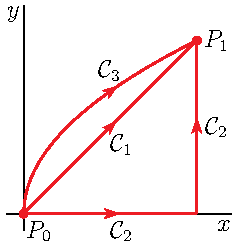
\includegraphics{workIntegralA.pdf}
\end{center}
\end{efig}
We shall calculate the work $\int_{\cC_i}\vF\cdot\dee{\vr}$ for each of 
the curves.
\begin{enumerate}[(a)]
\item 
We parametrize $\cC_1$ by $\vr(t) = t\,\hi+t\,\hj$ with $t$ running from $0$ to $1$.
Then $x(t)=t$ and $y(t)=t$ so that
\begin{equation*}
\vF\big(\vr(t)\big) = t^2\,\hi + (t^2+1)\,\hj\qquad\text{and}\qquad
\diff{\vr}{t}(t) = \hi + \hj
\end{equation*}
so that
\begin{align*}
\int_{\cC_1}\vF\cdot\dee{\vr}
&=\int_{0}^{1}\vF\big(\vr(t)\big)\cdot\diff{\vr}{t}(t)\,\dee{t}
=\int_{0}^{1}\big[t^2\,\hi + (t^2+1)\,\hj\big]\cdot[\hi + \hj]\,\dee{t} \\
&=\int_{0}^{1}\big[2t^2+1\big]\,\dee{t} \\
&=\frac{5}{3}
\end{align*}

\item 
We split $\cC_2$ into two parts, $\cC_{2,x}$ running from $P_0$ to $(1,0)$
along the $x$-axis and then $\cC_{2,y}$ running from $(1,0)$ to $P_1$
along the line $x=1$. 
We parametrize $\cC_{2,x}$ by $\vr(x) = x\,\hi$ with $x$ running from $0$ to $1$
and $\cC_{2,y}$ by $\vr(y) = \hi+y\,\hj$ with $y$ running from $0$ to $1$.
Then\footnote{You might like to think about why we can split up the integral like this.}
\begin{align*}
&\int_{\cC_2}\vF\cdot\dee{\vr}
=\int_{\cC_{2,x}}\vF\cdot\dee{\vr} + \int_{\cC_{2,y}}\vF\cdot\dee{\vr} \\
&\hskip0.25in=\int_{0}^{1}\big[(x) (0)\,\hi + (0^2+1)\,\hj\big]\cdot 
     \overbrace{\diff{\ }{x}\big(x\,\hi\big)}^{\hi}\,\dee{x}
 + \int_{0}^{1}\big[(1) (y)\,\hi + (y^2+1)\,\hj\big]\cdot 
           \overbrace{\diff{\ }{y}\big(\hi+y\,\hj\big)}^{\hj}\,\dee{y} \\
&\hskip0.25in=\int_{0}^{1}0\,\dee{x}
 + \int_{0}^{1}\big(y^2+1\big)\,\dee{y} \\
&\hskip0.25in=\frac{4}{3}
\end{align*}


\item 
We parametrize $\cC_3$ by $\vr(t) = t^2\,\hi+t\,\hj$ with $t$ running from $0$ to $1$.
Then $x(t)=t^2$ and $y(t)=t$ so that
\begin{equation*}
\vF\big(\vr(t)\big) = t^3\,\hi + (t^2+1)\,\hj\qquad\text{and}\qquad
\diff{\vr}{t}(t) = 2t\,\hi + \hj
\end{equation*}
so that
\begin{align*}
\int_{\cC_3}\vF\cdot\dee{\vr}
&%=\int_{0}^{1}\vF\big(t^2\,\hi+t\,\hj\big)\cdot\diff{\vr}{t}(t)\,\dee{t}
=\int_{0}^{1}\big[t^3\,\hi + (t^2+1)\,\hj\big]\cdot[2t\,\hi + \hj]\,\dee{t}
=\int_{0}^{1}\big[2t^4+t^2+1\big]\,\dee{t} \\
&=\frac{2}{5}+\frac{1}{3}+1 = \frac{26}{15}
\end{align*}
\end{enumerate}
Note that, despite the fact that $\cC_1$, $\cC_2$ and $\cC_3$ all start at $P_0$
and all end at $P_1$, the three integrals $\int_{\cC_1}\vF\cdot\dee{\vr}$, 
$\int_{\cC_2}\vF\cdot\dee{\vr}$ and $\int_{\cC_3}\vF\cdot\dee{\vr}$ all have different values.


\end{eg}

\begin{eg}\label{eg:workIntegalB}
Set\footnote{Again, the reader should verify that this vector field is not conservative.} 
\begin{equation*}
\vF(x,y) = 2y\,\hi + 3x\,\hj
\end{equation*}
This time we consider two curves.
\begin{enumerate}[(a)]
\item 
Let $\cC_1$ be circle $x^2+y^2=1$, traversed once counterclockwise, starting
at $(1,0)$.
\item 
Let $\cC_2$ be (trivial) curve which just consists of the single point $(1,0)$.
\end{enumerate}
We shall calculate the work $\int_{\cC_i}\vF\cdot\dee{\vr}$ for each 
curve.
\begin{enumerate}[(a)]
\item 
We parametrize $\cC_1$ by $\vr(t) = \cos t\,\hi+\sin t\,\hj$ with $t$ 
running from $0$ to $2\pi$, just as we did in Example \ref{eg:paramCircle}.
Then 
\begin{align*}
\oint_{\cC_1}\vF\cdot\dee{\vr}
&=\int_{0}^{2\pi}\big[2\sin t\,\hi + 3\cos t\,\hj\big]
           \cdot[-\sin t\,\hi + \cos t\,\hj]\,\dee{t}
=\int_{0}^{2\pi}\big[-2\sin^2 t+3\cos^2 t\big]\,\dee{t}
\end{align*}
You could evaluate these integrals using double angle trig identities
like you did in first year calculus. But there is a sneaky, much easier, way.
Because $\sin^2 t$ and $\cos^2 t$ are translates of each other, and both are
periodic of period $\pi$, the two integrals 
$\int_0^{2\pi}\sin ^2 t\,\dee{t}$ and $\int_0^{2\pi}\cos ^2 t\,\dee{t}$
represent the same area and so are equal. See the figure below. 
\begin{mfig}
\begin{center}
    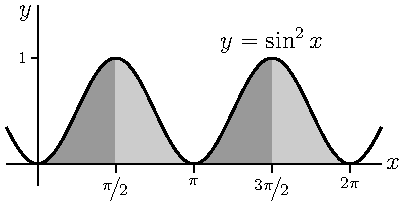
\includegraphics{sin2Graph.pdf}\qquad
    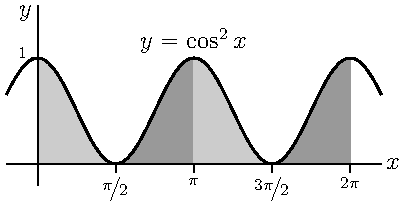
\includegraphics{cos2Graph.pdf}
\end{center}
\end{mfig}
Thus
\begin{align*}
\int_{0}^{2\pi} \sin^2 t\,\dee{t}
=\int_{0}^{2\pi} \cos^2 t\,\dee{t}
=\int_{0}^{2\pi} \frac{1}{2}\big[\sin^2 t+\cos^2t\big]\,\dee{t}
=\frac{1}{2}\int_{0}^{2\pi} \dee{t}
=\pi
\end{align*}
and 
\begin{align*}
\oint_{\cC_1}\vF\cdot\dee{\vr}
=-2\int_{0}^{2\pi} \sin^2 t\,\dee{t}
+3\int_{0}^{2\pi} \cos^2 t\,\dee{t}
=\pi
\end{align*}


\item 
We parametrize $\cC_2$ by $\vr(t) = \hi$ for all $t$. Then 
$\diff{\vr}{t}(t) = \vZero$ and $\int_{\cC_2}\vF\cdot\dee{\vr}=0$.


\end{enumerate}
Again, despite the fact that $\cC_1$ and $\cC_2$ both start at $(1,0)$
and end at $(1,0)$, the two integrals $\int_{\cC_1}\vF\cdot\dee{\vr}$ and 
$\int_{\cC_2}\vF\cdot\dee{\vr}$ are different.

\end{eg}

\begin{eg}[Example \ref{eg:screeningCounterexample}, again.]
                                        \label{eg:workIntegalC}
In Example \ref{eg:screeningCounterexample}, we saw that the vector field
\begin{equation*}
\vF(x,y) = -\frac{y}{x^2+y^2}\hi + \frac{x}{x^2+y^2}\hj
\qquad \text{defined for all $(x,y)$ in $\bbbr^2$ except $(x,y)=(0,0)$}
\end{equation*}
passed the screening test of Theorem \ref{thm:screen}.a, and yet was not 
conservative. In this example, we will see that this $\vF$ violates the 
conclusion of Theorem \ref{thm:workIntegral}, thereby providing a second proof
that $\vF(x,y)$ is not conservative on $\bbbr^2$ with $(0,0)$ removed.
For the curve $\cC$, of Theorem \ref{thm:workIntegral}, we use the circle 
parametrized by $x=a\cos\theta,\ y=a\sin\theta$, $0\le\theta\le 2\pi$. Then
$\dee{x}=-a\sin\theta\,\dee{\theta}$ and 
$\dee{y}=a\cos\theta\,\dee{\theta}$ so that
\begin{align*}
\frac{1}{2\pi}\int_\cC \frac{x\,\dee{y}-y\,\dee{x}}{x^2+y^2}
=\frac{1}{2\pi}\int_0^{2\pi} \frac{a^2\cos^2\theta\,\dee{\theta}+a^2\sin^2\theta\,\dee{\theta}}
             {a^2\cos^2\theta+a^2\sin^2\theta}
=\frac{1}{2\pi}\int_0^{2\pi}\dee{\theta}=1
\end{align*}
The curve $\cC$ has initial point 
\begin{align*}
P_0&=(a\cos\theta,\ a\sin\theta)\big|_{\theta=0} = (a,0)
\intertext{and final point} 
P_1&=(a\cos\theta,\ a\sin\theta)\big|_{\theta=2\pi} = (a,0) =P_0
\end{align*}
So, if $\vF$ were conservative with potential $\varphi$, 
Theorem \ref{thm:workIntegral} would give that 
\begin{equation*}
\frac{1}{2\pi}\int_\cC \frac{x\,\dee{y}-y\,\dee{x}}{x^2+y^2} 
=\varphi(P_1) - \varphi(P_0)=0
\end{equation*}
Consequently, $\vF$ can't be conservative. 
\end{eg}

\subsection{Path Independence}\label{sec:pathIndep}

This brings us to the following question. Let $\vF$ be any fixed vector field. 
When is it true that, given any two fixed points $P_0$ and $P_1$,
the integrals
\begin{equation*}
\int_{\cC}\vF\cdot\dee{\vr}=
\int_{\cC'}\vF\cdot\dee{\vr}
\end{equation*}
for all curves $\cC$, $\cC'$ that start at $P_0$ and end at $P_1$? 
When can we ignore the path taken? 
If this is the case we say that
``$\int_{\cC}\vF\cdot\dee{\vr}$ is independent of the path chosen'' 
and we write
\begin{equation*}
\int_{P_0}^{P_1}\vF\cdot\dee{\vr}
=\int_{\cC}\vF\cdot\dee{\vr}
\end{equation*}
for any path $\cC$ from $P_0$ to $P_1$.
The point of this section is that there is an intimate relation between
path independence and conservativeness of vector fields, that we will
get to in Theorem \ref{thm:pathIndepConserv}.

 For simplicity, we will consider only vector fields that are defined and continuous on all of $\bbbr^2$
(i.e. the $xy$-plane) or $\bbbr^3$ (i.e. the usual three dimensional world).
Some discussion about what happens for vector fields that are defined only 
on part of $\bbbr^2$ or $\bbbr^3$ is given in the optional 
\S\ref{sec:cohomology}. 

First we show that if there is one pair of (not necessarily distinct)
points $P_0$, $P_1$ such that
\begin{equation*}
\int_{\cC_1}\vF\cdot\dee{\vr}=
\int_{\cC_2}\vF\cdot\dee{\vr}
\end{equation*}
for all curves $\cC_1$, $\cC_2$ that start at $P_0$ and end at $P_1$,
then it is also true that, for \emph{any} other pair of points 
$P_0'$, $P_1'$
\begin{equation*}
\int_{\cC'_1}\vF\cdot\dee{\vr}=
\int_{\cC'_2}\vF\cdot\dee{\vr}
\end{equation*}
for all curves $\cC'_1$, $\cC'_2$ that start at $P'_0$ and end at $P'_1$.
This might seem unlikely at first, but the idea of the proof is really 
intuitive.


\begin{theorem}\label{thm:pathIndepArbEndPoints}
Let $\vF$ be a vector field that is defined and continuous on all of $\bbbr^2$
(or $\bbbr^3$). Let $P_0$, $P_1$, $P'_0$, $P'_1$ be any four points 
in $\bbbr^2$ (or $\bbbr^3$). Assume that 
\begin{equation*}
\int_{\cC_1}\vF\cdot\dee{\vr}=
\int_{\cC_2}\vF\cdot\dee{\vr}
\end{equation*}
for all curves $\cC_1$, $\cC_2$ that start at $P_0$ and end at $P_1$.
Then
\begin{equation*}
\int_{\cC'_1}\vF\cdot\dee{\vr}=
\int_{\cC'_2}\vF\cdot\dee{\vr}
\end{equation*}
for all curves $\cC'_1$, $\cC'_2$ that start at $P'_0$ and end at $P'_1$.
\end{theorem}
\begin{proof}
Let $\cC'_1$ and $\cC'_2$ be any two curves that start at $P'_0$ and 
end at $P'_1$. 
\vadjust{
\begin{efig}
\begin{center}
    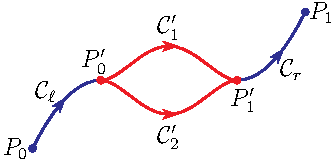
\includegraphics{pathIndep.pdf}
\end{center}
\end{efig}
}
We start by choosing any two (auxiliary) curves 
\begin{itemize}\itemsep1pt \parskip0pt \parsep0pt %\itemindent-15pt
\item[$\circ$]
$\cC_\ell$ that starts at $P_0$ and ends at $P'_0$ and
\item[$\circ$]
$\cC_r$ that starts at $P'_1$ and ends at $P_1$.
\end{itemize}
and then we define the curves 
\begin{itemize}\itemsep1pt \parskip0pt \parsep0pt %\itemindent-15pt
\item[$\circ$]
$\cC_1$ to be $\cC_\ell$, followed by $C'_1$, followed by $\cC_r$ and
\item[$\circ$]
$\cC_2$ to be $\cC_\ell$, followed by $C'_2$, followed by $\cC_r$.
\end{itemize}
Then both $\cC_1$ and $\cC_2$ start at $P_0$ and end at $P_1$, so that, 
by hypothesis,
\begin{equation*}
\int_{\cC_1}\vF\cdot\dee{\vr}=
\int_{\cC_2}\vF\cdot\dee{\vr}
\end{equation*}
and, from the construction of $\cC_1$ and $\cC_2$,
\begin{align*}
&\int_{\cC_\ell}\vF\cdot\dee{\vr}
+\int_{\cC'_1}\vF\cdot\dee{\vr}
+\int_{\cC_r}\vF\cdot\dee{\vr}=
\int_{\cC_\ell}\vF\cdot\dee{\vr}
+\int_{\cC'_2}\vF\cdot\dee{\vr}
+\int_{\cC_r}\vF\cdot\dee{\vr} \\
\implies & \int_{\cC'_1}\vF\cdot\dee{\vr}=
\int_{\cC'_2}\vF\cdot\dee{\vr}
\end{align*}
as desired.
\end{proof}

We are now ready for our main theorem on conservative fields.
\begin{theorem}\label{thm:pathIndepConserv}
Let $\vF$ be a vector field that is defined and continuous on all of $\bbbr^2$
(or $\bbbr^3$). Then the following three statements are equivalent.
\begin{enumerate}[(a)]
\item
$\vF$ is conservative. That is, there exists a function $\varphi$ such that
$\vF=\vnabla\varphi$.
\item
The integral $\oint_\cC\vF\cdot\dee{\vr}=0$ for any closed curve $\cC$.

\item
The integral $\int\vF\cdot\dee{\vr}$ is path independent. That is,
for any points $P_0$, $P_1$ we have 
$
\int_{\cC_1}\vF\cdot\dee{\vr}=
\int_{\cC_2}\vF\cdot\dee{\vr}
$
for all curves $\cC_1$, $\cC_2$ that start at $P_0$ and end at $P_1$.
\end{enumerate}
That is, if any one of the three statements are true, then all three are true.
\end{theorem}
\begin{proof}
It suffices for us to prove\footnote{This is a pretty efficient, and 
standard, way to structure the proof of the equivalence of three 
statements.} that 
\begin{itemize}\itemsep1pt \parskip0pt \parsep0pt %\itemindent-15pt
\item[$\circ$]
the truth of (a) implies the truth of (b) and
\item[$\circ$]
the truth of (b) implies the truth of (c) and
\item[$\circ$]
the truth of (c) implies the truth of (a).
\end{itemize}
That's exactly what we will do.

\noindent (a)$\implies$(b):\ \ \ 
Let $\cC$ be a closed curve that starts at $P_0$ and then ends back at $P_0$.
Then, by Theorem \ref{thm:workIntegral} with $P_1=P_0$,
\begin{equation*}
\oint_\cC\vF\cdot\dee{\vr} =\varphi(P_0) - \varphi(P_0)=0
\end{equation*}

\noindent (b)$\implies$(c):\ \ \ 
Pick any point $P_0$ and set $P_1=P_0$. Then we are assuming that
$\oint_\cC\vF\cdot\dee{\vr}=0$ for all curves that start at $P_0$ and end at $P_1$.
In particular  $\int_\cC\vF\cdot\dee{\vr}$ takes the same value for all curves
that start at $P_0$ and end at $P_1$.
So Theorem \ref{thm:pathIndepArbEndPoints} immediately yields
property (c).

\medskip
\noindent (c)$\implies$(a):\ \ \ We are to show that $\vF$ is conservative.
We'll start by guessing $\varphi$ and then we'll verify that, for our
chosen $\varphi$, we really do have $\vF=\vnabla\varphi$. Our guess for 
$\varphi$ is motivated by Theorem \ref{thm:workIntegral}. If our $\vF$ really is conservative, its potential is going to have to obey
$\int_\cC\vF\cdot\dee{\vr} =\varphi(P_1) - \varphi(P_0)$ for any curve $\cC$ that starts at $P_0$ and ends at $P_1$. Let's choose $P_0=\vZero$. Remembering,
from Definition \ref{def:conservative}.a, that adding a constant to a 
potential always yields another potential, we can always choose 
$\varphi(\vZero)=0$. Then $\varphi(P_1)=\int_\cC\vF\cdot\dee{\vr}$ for any 
curve $\cC$ that starts at $\vZero$ and ends at $P_1$. So define,
for each point $\vx$, $\varphi(\vx)=\int_\cC\vF\cdot\dee{\vr}$ for any 
curve $\cC$ that starts at $\vZero$ and ends at $\vx$.

We now verify that, for this chosen $\varphi$, we really do have $\vF=\vnabla\varphi$.
Fix any point $\vx$ and any curve $\cC_{\vx}$ that
starts at the origin and ends at $\vx$. 
For any vector $\vu$, let $\cD_{\vu}$ be the curve with parametrization
\begin{equation*}
\vr_{\vu}(t)=\vx+t\vu\qquad 0\le t\le 1
\end{equation*}
This curve is a line segment that starts at $\vx$ at $t=0$ and ends at $\vx+\vu$ at $t=1$.
Observe that ${\vr\,}'_{\vu}(t)=\vu$.
Recall that, by assumption, $\varphi(\vx+s\vu)=\int_\cC\vF\cdot\dee{\vr}$ for \emph{any} 
curve $\cC$ that starts at $\vZero$ and ends at $\vx+s\vu$. So
\begin{equation*}
\varphi(\vx+s\vu)
=\int_{\cC_{\vx}+\cD_{s\vu}}\vF\cdot d\vr
\end{equation*}
where $C_{\vx}+D_{s\vu}$ is the curve which first follows 
$C_{\vx}$ from the origin to $\vx$ and then follows $D_{s\vu}$
from $x$ to $\vx+s\vu$. We have
\begin{align*}
\int_{C_{\vx}+D_{s\vu}}\vF\cdot d\vr
&=\int_{C_{\vx}}\vF\cdot d\vr
+\int_{D_{s\vu}}\vF\cdot d\vr \\
&=\int_{C_{\vx}}\vF\cdot d\vr
+\int_0^1 \vF(\vx+ts\vu)\cdot (s\vu)\,dt
\end{align*}
In the second integral, make the change of variables 
$\tau=ts$, $\dee{\tau}=s\dee{t}$. This  gives 
\begin{equation*}
\varphi(\vx+s\vu)=\int_{C_{\vx}}\vF\cdot d\vr
+\int_0^s \vF(\vx+\tau\vu)\cdot \vu\,d\tau
\end{equation*}
By the fundamental theorem of calculus, applied to the second integral,
\begin{equation*}
\diff{\ }{s}\varphi(\vx+s\vu)\Big|_{s=0}
=\vF(\vx+s\vu)\cdot \vu\Big|_{s=0}=\vF(\vx)\cdot \vu
\end{equation*}
Applying this with $\vu=\hi,\ \hj,\ \hk$ gives us
\begin{equation*}
\Big(\frac{\partial\varphi}{\partial x}(\vx)\,,\,
     \frac{\partial\varphi}{\partial y}(\vx)\,,\,
     \frac{\partial\varphi}{\partial z}(\vx)\Big) 
=\big(\vF(\vx)\cdot\hi\,,\,\vF(\vx)\cdot\hj\,,\,\vF(\vx)\cdot\hk\big)
\end{equation*}
which is
\begin{equation*}
\nabla\varphi(\vx)=\vF(\vx)
\end{equation*}
as desired.
\end{proof}
Using this result, we can completely characterize conservative fields on
$\bbbr^2$ and $\bbbr^3$.

\begin{theorem}\label{thm:screenConserv}
Let $\vF$ be a vector field that is defined and has continuous 
first order partial derivatives on all of $\bbbr^2$ (or $\bbbr^3$).
Then $\vF$ is conservative if and only if it passes the screening test
$\vnabla\times\vF=\vZero$, i.e. is curl free.
\end{theorem}
\begin{warning}\label{warn:screeningB}
Note that in Theorem \ref{thm:screenConserv} we are assuming that
$\vF$ passes the screening test on \emph{all} of $\bbbr^2$ or $\bbbr^3$.
We have already seen, in Example \ref{eg:screeningCounterexample},
that if the screening test fails at even a single point, for example
because the vector field is not defined at that point, then $\vF$ need 
not be conservative. We'll explore what happens in such cases in the
(optional)  \S\ref{sec:cohomology}. We'll see that something can be salvaged.
\end{warning}

\begin{proof}[Proof of Theorem \ref{thm:screenConserv}]
We'll give the proof for the $\bbbr^2$ case. The proof for the $\bbbr^3$ case
is very similar.
We have already seen, in Theorem \ref{thm:screen}, that if $\vF$ 
is conservative, then it passes the screening test and there is nothing more
to do. 

So we now have 
to assume that $\vF$ obeys $\frac{\partial F_1}{\partial y}(x,y) 
=  \frac{\partial F_2}{\partial x}(x,y)$ on \emph{all} of $\bbbr^2$
and prove that it is conservative. We'll do so 
using the strategy of Example \ref{eg:potentialD} to find a function
$\varphi(x,y)$, that obeys
\begin{equation*}%\label{eqn:screenConservS}
\begin{split}
\frac{\partial \varphi}{\partial x}(x,y) &= F_1(x,y) \\
\frac{\partial \varphi}{\partial y}(x,y) &= F_2(x,y)
\end{split}
\end{equation*}
The partial derivative $\frac{\partial \ }{\partial x}$ treats $y$
as a constant. So $\varphi(x,y)$ obeys the first equation
if and only if there is a function $\psi(y)$ with
\begin{equation*}
\varphi(x,y)
=\int_0^x F_1(X,y)\,\dee{X}
\ +\ \psi(y)
\end{equation*}
This $\varphi(x,y)$ will also obey the second equation if and only if 
\begin{align*}
F_2(x,y)&= \frac{\partial \varphi}{\partial y}(x,y)\\
&=\frac{\partial \ }{\partial y}\Big(\int_0^x F_1(X,y)\,\dee{X}\ +\ \psi(y)\Big)
\\
&=\int_0^x \frac{\partial F_1}{\partial y}(X,y)\,\dee{X}\ +\ \psi'(y)
\end{align*}
So we have to find a $\psi(y)$ that obeys
\begin{equation*}
\psi'(y) = F_2(x,y) - 
                \int_0^x \frac{\partial F_1}{\partial y}(X,y)\,\dee{X}
\end{equation*}
This looks bad --- no matter what $\psi(y)$ is, the left hand side is 
independent of $x$, while it looks like the right hand side depends on $x$. 
Fortunately our screening test hypothesis now rides in to the 
rescue\footnote{or bails us out, or saves our bacon, or $\ldots$}.
(We haven't used it yet, and it has to come in somewhere.)
\begin{align*}
F_2(x,y) -  \int_0^x \frac{\partial F_1}{\partial y}(X,y)\,\dee{X}
&=F_2(x,y) -  \int_0^x \frac{\partial F_2}{\partial x}(X,y)\,\dee{X} \\
&= F_2(x,y) - F_2(X,y)\Big|_{X=0}^{X=x} \\
&=F_2(0,y)
\end{align*}
In going from the first line to the second line we used 
the fundamental theorem of calculus. So choosing
\begin{equation*}
\psi(y) = \int_0^y F_2(0,Y)\,\dee{Y} +C
\end{equation*}
for any constant $C$, does the trick.
\end{proof}


\section{Optional --- The Pendulum}\label{sec:Pendulum}

Model a pendulum by a mass $m$ that is connected to a hinge by 
an idealized rod that is massless and of fixed length $\ell$. Denote 
by $\theta$ the angle
\vadjust{
\begin{efig}
\begin{center}
    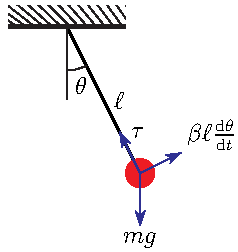
\includegraphics{pendulum2.pdf}\qquad\qquad
    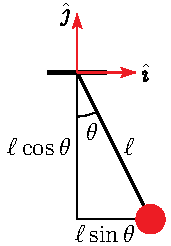
\includegraphics{pendulum4.pdf}
\end{center}
\end{efig}
}
between the rod and vertical. The forces acting on the mass are
\begin{itemize}\itemsep1pt \parskip0pt \parsep0pt %\itemindent-15pt
\item[$\circ$]
gravity, which has magnitude $mg$ and direction $(0,-1)$, 
\item[$\circ$]
tension in the rod, whose magnitude, $\tau$, automatically adjusts 
itself so that the distance between the mass and the hinge is 
fixed at $\ell$ and whose direction,
$(-\sin\theta,\cos\theta)$, is always parallel to the rod and 
\item[$\circ$]
possibly some frictional forces, like friction in the hinge and 
air resistance. We shall assume that the total frictional force 
has magnitude proportional to the speed\footnote{The dependence of air resistance (drag) on the speed $v$ is relatively complex. At low speed 
drag tends to be approximately proportional to $v$, while at high speed 
it tends to be approximately proportional to $v^2$.} of the 
mass and has direction opposite to the direction of motion of the mass.
\end{itemize}
If we use a coordinate system centered on the hinge, the $(x,y)$ 
coordinates of the mass at time $t$ are 
$\ell\big(\sin\theta(t),-\cos\theta(t)\big)$. 
Hence its  velocity vector is 
\begin{equation*}
\vv(t)
 = \diff{\ }{t}\big[\ell\big(\sin\theta(t),-\cos\theta(t)\big) \big]
  = \ell\big(\cos\theta(t),\sin\theta(t)\big)\diff{\theta}{t}(t)
\end{equation*}
and the  total frictional force is 
$-\be \ell(\cos\theta,\sin\theta)\diff{\theta}{t}$,
for some constant $\be$.
The acceleration vector of the mass is
\begin{equation*}
\va(t)=\diff{\ }{t}\vv(t)
=\ell(\cos\theta,\sin\theta)\difftwo{\theta}{t}
+\ell(-\sin\theta,\cos\theta)\Big(\diff{\theta}{t}\Big)^2
\end{equation*}
so that Newton's law of motion, $\vF=m\va$,  now tells us
\begin{align*}
m\va(t) &= m\ell(\cos\theta,\sin\theta)\difftwo{\theta}{t}
+m\ell(-\sin\theta,\cos\theta)\Big(\diff{\theta}{t}\Big)^2\\
&=\vF=mg(0,-1)+\tau (-\sin\theta,\cos\theta)
-\be \ell(\cos\theta,\sin\theta)\diff{\theta}{t}
\end{align*}
To eliminate the (unknown) coefficient $\tau$ we dot this equation with
$(\cos\theta,\sin\theta)$, which extracts 
the component parallel to the direction of motion of the 
mass. Dotting with $(\cos\theta,\sin\theta)$ gives
$\ 
m\ell\difftwo{\theta}{t}=-mg\sin\theta-\be \ell\diff{\theta}{t}
\ $
or
\begin{equation*}
\difftwo{\theta}{t}+\frac{\be}{m}\diff{\theta}{t}
              +\frac{g}{\ell}\sin\theta=0
\end{equation*}
which is the equation of motion of the (nonlinear) pendulum. 
In general, it can be hard to analyse nonlinear differential 
equations. But if the amplitude of oscillation is small enough 
that we may approximate 
$\sin\theta$ by $\theta$ we get the equation of motion 
of the linear pendulum\footnote{When $\be=0$, this equation reduces
to the equation $\difftwo{\theta}{t}+\frac{g}{\ell}\theta=0$, which occurs 
in many different applications, and whose solutions exhibit simple 
harmonic motion.} which is 
\begin{align*}
\difftwo{\theta}{t}+\frac{\be}{m}\diff{\theta}{t}
+\frac{g}{\ell}\theta=0
\end{align*}
These equations may be reformulated as systems of first order 
ordinary differential equation, that is as equations for the 
flow lines of a vector field, by the simple expedient of 
defining (as we did in Example \ref{eg:Pendulum})
\begin{equation*}
x(t)=\theta(t)\qquad y(t)=\theta'(t)
\end{equation*}
Then, for the full, nonlinear, equation 
$ \difftwo{\theta}{t}+\frac{\be}{m}\diff{\theta}{t}
+\frac{g}{\ell}\sin\theta=0$
\begin{alignat*}{3}
x'(t)&=&\theta'(t)&=y(t)\cr
y'(t)&=&\ \theta''(t)&=-\frac{g}{\ell}\sin x(t)-\frac{\be}{m} y(t)
\end{alignat*}
The solutions of this first order system of ordinary differential equations
are flow lines for the vector field
\begin{equation*}
\vV\big((x,y)\big)=\Big(y\,,\,-\frac{g}{\ell}\sin x-\frac{\be}{m} y\Big)
\end{equation*}
When $\be=0$, this is exactly the vector field of Example \ref{eg:Pendulum}.











